\documentclass[10pt,letterpaper,final]{report}

% Paquetes
\usepackage[utf8]{inputenc}
\usepackage[spanish]{babel}
\usepackage{amsmath}
\usepackage{amssymb} % Blackboard bold (\mathbb)
\usepackage{graphicx}
\usepackage{svg} % Para incluir gráficos SVG
\usepackage{hyperref}
\usepackage{tocbibind} % Para incluir referencias en el índice
\usepackage{caption}
\usepackage{subcaption} % Paquete para justificar el texto


%% Various layout settings: may require adjustment

\makeatletter
%page layout
\@twosidefalse 
% distance from top of page to page's head
\topmargin -0.35in      % head margin = .75in or 2cm
% distance between the left side and text left margin
\oddsidemargin 0.5in    % binding margin = 1.5in or 4cm

\headheight 20pt 
\headsep 15pt
%\footheight 48pt    % this line doesn't work in latex2e
\footskip 28pt
\textheight 9.05in 
\textwidth 5.68in
\parskip 8pt
\parindent 10pt
\columnwidth \textwidth
\footnotesep 12pt

%floats and marginpar
\floatsep 12pt plus 2pt minus 2pt
\textfloatsep  20pt plus 2pt minus 4pt
\intextsep 12pt plus 2pt minus 2pt
\dblfloatsep 12pt plus 2pt minus 2pt
\dbltextfloatsep 20pt plus 2pt minus 4pt
%\@maxsep 20pt     % this line doesn't work in latex2e
%\@dblmaxsep 20pt  % this line doesn't work in latex2e
\@fptop 0pt plus 1fil
\@fpsep 8pt plus 2fil
\@fpbot 0pt plus 1fil
\@dblfptop 0pt plus 1fil
\@dblfpsep 8pt plus 2fil
\@dblfpbot 0pt plus 1fil
\marginparwidth 90pt
\marginparsep 11pt
\marginparpush 5pt
\makeatother
%% End of layout settings.

% Following modified from article.doc to put a little indentation between
% the footnote marker and the text of the footnote
% The change is the explicit blank just before the second $ sign
% This can be removed if you prefer ugly footnotes.

\makeatletter
\long\def\@makefntext#1{\@setpar{\@@par\@tempdima \hsize
  \advance\@tempdima-10pt\parshape \@ne 10pt \@tempdima}\par
  \parindent 1em \hbox to \z@{\hss$^{\@thefnmark}\ $}#1}
\makeatother

% Some commands to handle linespacing

\newlength{\spacing}
\setlength{\spacing}{\baselineskip}

\newcommand{\nspace}[1]{\setlength{\baselineskip}{#1\spacing}}
\newenvironment{linespacing}[1]{\nspace{#1}}{}


% Información del documento
\title{Estimación de la pose de un vehículo mediante cámaras y sensores para estacionamiento automático en simulación}
\author{Ing. Rubén Martínez González}
\date{Septiembre 2025}
\newcommand{\university}{Universidad Autónoma de Yucatán}
\newcommand{\faculty}{Facultad de Matemáticas}
\newcommand{\advisor}{Dr. Arturo Espinosa Romero}
\newcommand{\myauthor}{Ing. Rubén Martínez González}
\newcommand{\degree}{Maestría en Ciencias de la Computación}
\newcommand{\tesisInv}{Tesis de investigación}
\newcommand{\mydate}{Septiembre 2025}
\newcommand{\mytitle}{Estimación de la pose de un vehículo mediante cámaras y sensores para estacionamiento automático en simulación}

\begin{document}

% Portada moderna
\begin{titlepage}
    \centering
    % Logos
    \begin{minipage}{0.25\textwidth}
        \centering
        
\includegraphics[width=0.8\textwidth]{img/fmat.png}
    \end{minipage}%
    \hfill
    \begin{minipage}{0.5\textwidth}
        \centering
        {\scshape\small \university \par}
        \vspace{0.2cm}
        {\scshape\small \faculty \par}
        \vspace{0.2cm}
        {\scshape\small \degree \par}
    \end{minipage}%
    \hfill
    \begin{minipage}{0.25\textwidth}
        \centering
        
\includegraphics[width=0.8\textwidth]{img/UADY.jpg}
    \end{minipage}

    \vspace{1.5cm}
    {\LARGE\bfseries \mytitle \par}
    \vspace{1.5cm}
    {\Large \tesisInv \par}
    \vspace{1cm}
    {\large Autor: \textbf{\myauthor}\par}
    \vspace{0.5cm}
    {\large Asesor: \textbf{\advisor}\par}
    \vfill
    \vspace{0.5cm}
    {\large \mydate \par}
\end{titlepage}

% Resumen
\begin{abstract}
    \noindent
Este documento presenta un enfoque para la estimación de la posición de un vehículo en un entorno de estacionamiento
utilizando técnicas de visión por computadora y aprendizaje automático. Se describe la implementación de un sistema
de simulación que permite la recolección de datos de sensores y la generación de imágenes sintéticas para entrenar 
modelos de detección de objetos. Los resultados muestran la efectividad del enfoque propuesto en la identificación de 
espacios de estacionamiento y la navegación autónoma en entornos complejos.
\end{abstract}
\clearpage


% Índice
\tableofcontents
\listoffigures
\clearpage

\begin{linespacing}{1.5}

% Capítulo 1: Introducción
\chapter{Introducción}
\noindent
El estacionamiento es una actividad esencial en la vida urbana, ya que permite a los conductores dejar sus vehículos en reposo mientras realizan otras actividades.
No obstante, el estacionamiento en áreas urbanas congestionadas presenta múltiples desafíos, incluyendo la falta de espacio,
la presencia de obstáculos y la visibilidad reducida, lo cual incrementa el riesgo de colisiones y daños a los vehículos.
Incluso habiendo identificado el espacio de estacionamiento, el proceso de maniobrar el vehículo para estacionar puede ser complicado y estresante,
especialmente para conductores con poca experiencia o en vehículos grandes.\\
\noindent
Para mitigar estos problemas, se han desarrollado sistemas avanzados de asistencia al conductor, como el estacionamiento automático,
que facilitan esta tarea y mejoran la seguridad.
Sin embargo, la efectividad de estos sistemas depende en gran medida de la capacidad para estimar con precisión la posición del vehículo
con respecto al espacio de estacionamiento.
Una estimación incorrecta puede resultar en maniobras inseguras, especialmente en entornos con espacio limitado.\\
\noindent
Representar esta ubicación de manera adecuada es crucial para el desarrollo de un sistema de estacionamiento automático confiable.
Para abordar esta cuestión, se propone diseñar una simulación en donde se obtendrán datos de sensores
y cámaras del vehículo para estimar su posición relativa al espacio de estacionamiento.\\
\noindent
La simulación se llevará a cabo en un entorno controlado que refleja las condiciones reales de estacionamiento.
%Se modelará un escenario de estacionamiento con un vehículo y su espacio de estacionamiento, donde se adquirirán datos de sensores.
Dicho entorno consistirá de un cajón de estacionamiento objetivo, el vehículo que se va a controlar y objetos estáticos que pueden generar oclusiones.
El entorno de simulación permitirá extraer información a través de sensores los cuales permitirán hacer mediciones de las distancias y ángulos necesarios para maniobrar durante el estacionamiento.\\
\noindent
Las mediciones obtenidas, representadas mediante coordenadas cilíndricas, proporcionarán la información necesaria para entrenar algoritmos de aprendizaje automático.
Estos algoritmos podrán aprender y adaptarse a diversas condiciones y escenarios, mejorando la precisión y seguridad del sistema de estacionamiento automático.\\
\noindent
La investigación se centra en desarrollar un sistema que, mediante la estimación de la posición del vehículo y la simulación de este entorno, permita avanzar en la creación de sistemas de estacionamiento automático eficientes y seguros en entornos urbanos congestionados.

\section{Contexto y problemática}
\noindent
%    problemas en los estacionamientos
Los estacionamientos son imprescindibles en la vía urbana, ya que permiten a los conductores estacionar sus vehículos
de manera segura y eficiente. Sin embargo, el proceso de estacionamiento puede ser complicado y estresante,
especialmente en áreas congestionadas con espacio limitado y visibilidad reducida.
Factores como la falta de espacio, la presencia de obstáculos y la poca visibilidad para el conductor ocasionan
dificultades al estacionar un vehículo, lo que puede aumentar el riesgo de colisiones y daños al vehículo.
\\
%   se han logrado sistemas de asistencia al conductor
En la actualidad, la búsqueda de soluciones para mejorar la eficiencia y seguridad en el desplazamiento vehicular
ha llevado al desarrollo de sistemas avanzados de asistencia al conductor.
Entre estos sistemas, el estacionamiento automático ha ganado relevancia como una función que puede contribuir
a reducir los riesgos asociados con el estacionamiento en entornos urbanos congestionados.
\\
%   problemas de sistemas de estacionamiento automático
Sin embargo, el desarrollo de sistemas de estacionamiento automático presenta desafíos significativos,
especialmente en lo que respecta a la estimación de la posición del vehículo con respecto al espacio de estacionamiento.
El cálculo incorrecto de esta posición puede resultar en maniobras de estacionamiento inseguras o peligrosas,
especialmente en entornos donde el espacio de estacionamiento es limitado o con poca visibilidad para el conductor.
\\
%   necesidad de sistemas de asistencia al conductor más autónomos
En este contexto, continua la necesidad de desarrollar soluciones de utilidad para que los sistemas de asistencia al conductor
sean cada vez más autosuficientes y no dependan de la intervención limitada del conductor.
\\
%   en que consiste la investigación
Esta investigación se enfoca en poder estimar la posición de un vehículo con respecto a su espacio de estacionamiento
utilizando cámaras y sensores y utilizar esta posición estimada para lograr un sistema de estacionamiento automático en simulación.

\section{Preguntas de investigación}

\begin{itemize}
    \item ¿Cómo se puede representar la posición de un vehículo con respecto a su espacio de estacionamiento?
    \item ¿Cómo se puede estimar esta posición utilizando las cámaras y sensores del vehículo?
    \item ¿Cómo usar esta posición estimada para que el vehículo se estacione automáticamente?
\end{itemize}

\subsection{Hipótesis}
\noindent
``Estimando la posición relativa al estacionamiento de un vehículo mediante cámaras y sensores,
y utilizando esta posición, se puede lograr un sistema de estacionamiento automático en simulación.''


\section{Objetivos}
\subsection{Objetivo General}
\noindent
Desarrollar un sistema de estimación de la posición relativa al estacionamiento de un vehículo mediante cámaras y sensores para estacionamiento automático.

\subsection{Objetivos específicos}
\noindent
\begin{itemize}
    \item Modelar un ambiente de simulación de un vehículo y estacionamiento.
    \item Obtener datos de los sensores del vehículo en simulación.
    \item Interpretar los datos de los sensores mediante técnicas de visión computacional.
    \item Procesar los datos y estimar la posición del vehículo con respecto al estacionamiento.
    \item Utilizar la posición estimada para lograr un sistema de estacionamiento automático en simulación.
\end{itemize}

\section{Estado del arte - Trabajos previos relacionados}
\noindent\textbf{Autonomous Driving Architectures: Insights of Machine Learning and Deep Learning Algorithms}~\cite{bachute2021autonomous}
El artículo fue publicado en la revista Machine Learning with Applications en 2021 y
proporciona una visión general de la aplicación de algoritmos de Aprendizaje Automático y Aprendizaje Profundo
en sistemas de conducción autónoma, destacando su evaluación en tareas cruciales.
Se destaca el creciente impulso en la investigación de la conducción autónoma debido a sus ventajas inherentes, como la reducción
de la intervención humana y la disociación del conductor del vehículo.
Se subraya la complejidad de estos sistemas,
que involucra la integración de múltiples subsistemas, y se analizan diversas tareas específicas dentro de la conducción autónoma,
como la planificación de movimiento, la detección de peatones y señales de tráfico, el estacionamiento automatizado, entre otras.
El estudio se centra en la aplicación de algoritmos de Aprendizaje Automático y Aprendizaje Profundo para abordar estas tareas,
evaluando y comparando su rendimiento a través de métricas específicas. La investigación ofrece una perspectiva amplia sobre el uso
y la evaluación en el contexto de la conducción autónoma.
\begin{figure}[!ht]
    \centering
    \begin{subfigure}{0.4\textwidth}
        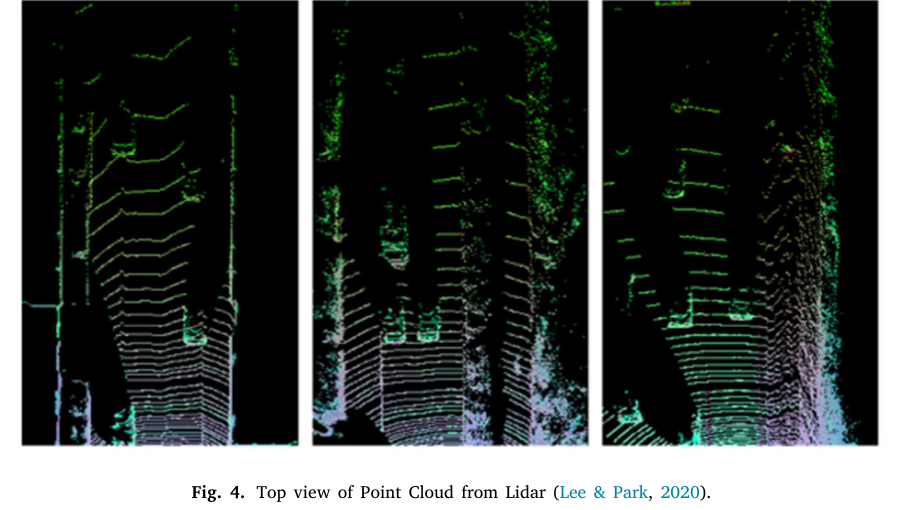
\includegraphics[width=\textwidth]{img/12Screenshot_20231106_142954}\label{fig:12}
    \end{subfigure}
    \begin{subfigure}{0.4\textwidth}
        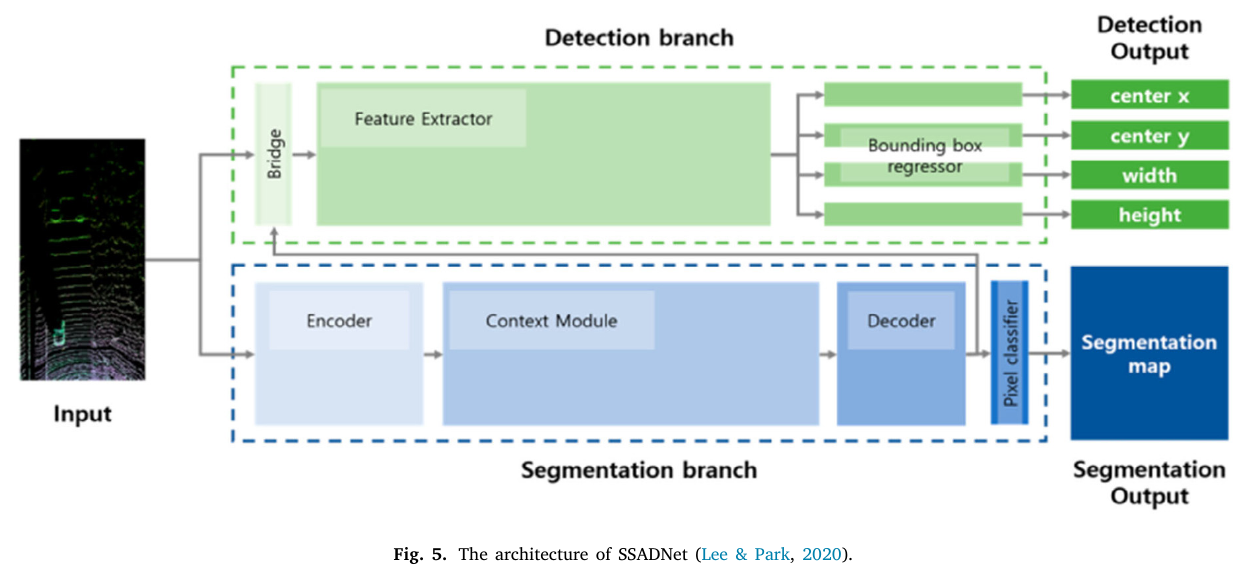
\includegraphics[width=\textwidth]{img/13Screenshot_20231106_143018}\label{fig:13}
    \end{subfigure}
    \begin{subfigure}{0.4\textwidth}
        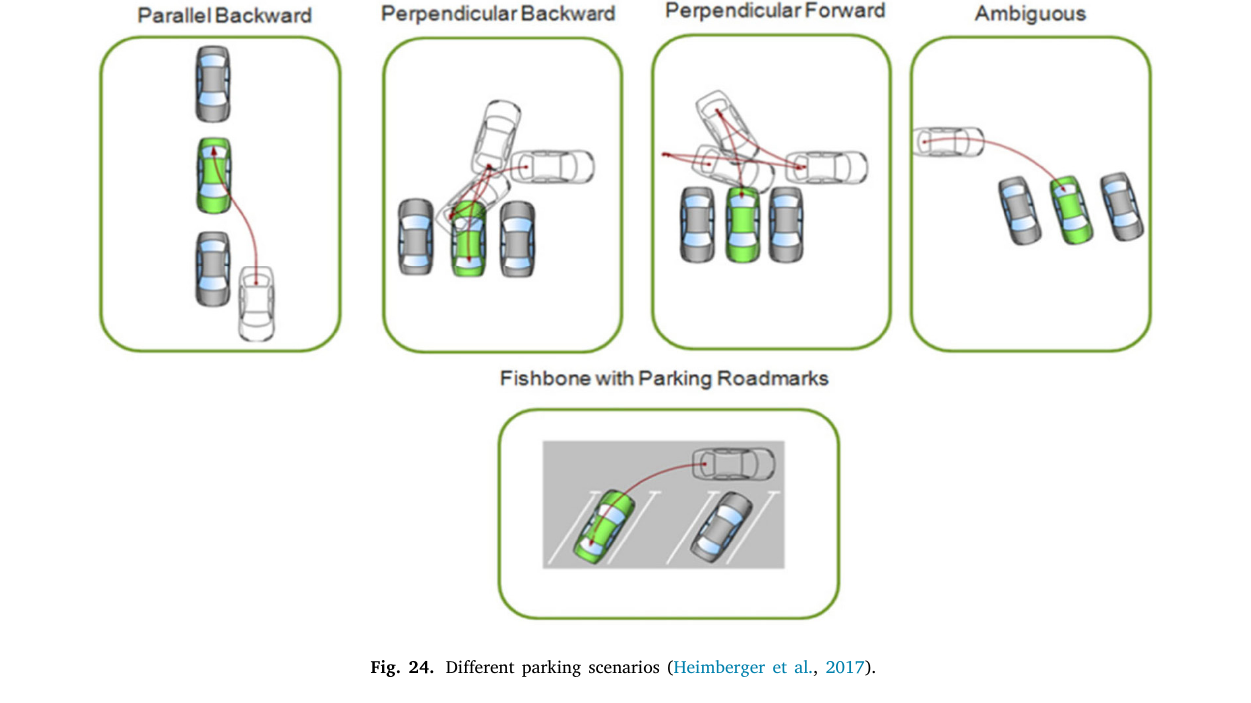
\includegraphics[width=\textwidth]{img/15Screenshot_20231106_143633}\label{fig:15}
    \end{subfigure}
    \begin{subfigure}{0.5\textwidth}
        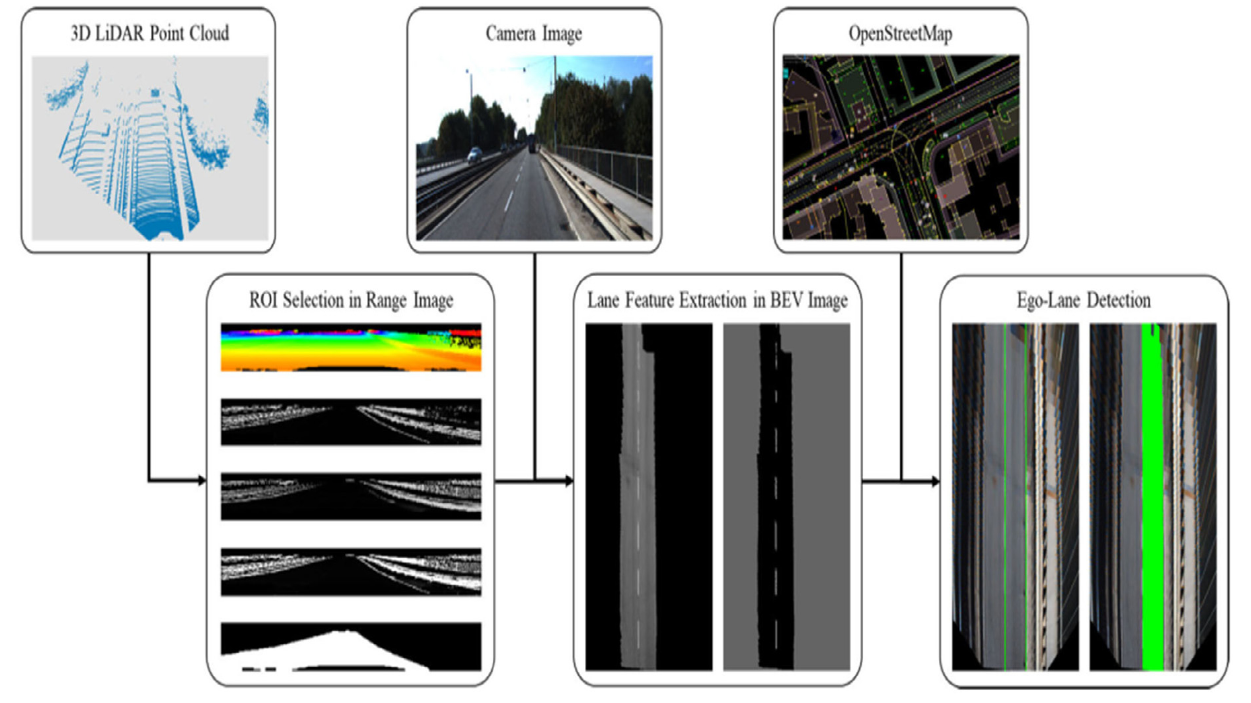
\includegraphics[width=\textwidth]{img/14 Screenshot_20231106_143419}\label{fig:14}
    \end{subfigure}
    \begin{subfigure}{\textwidth}
        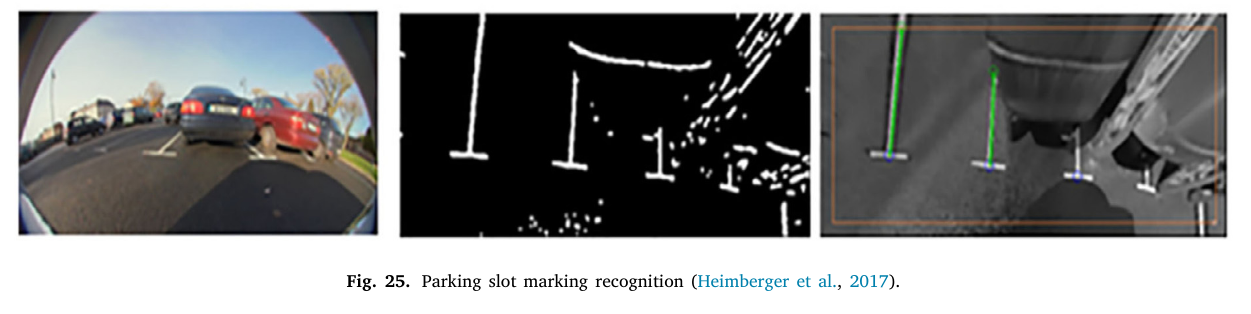
\includegraphics[width=0.99\textwidth]{img/16Screenshot_20231106_143701}\label{fig:16}
    \end{subfigure}
\end{figure}
\clearpage

\noindent\textbf{Vision-based autonomous car racing using deep imitative reinforcement learning}~\cite{cai2021vision}
El artículo fue publicado en la revista IEEE Robotics and Automation Letters en 2021 y aborda el desafío del automovilismo autónomo
en el campo del control robótico, históricamente dependiente de mapas precisos, localización y planificación, lo que lo hace
computacionalmente ineficiente y sensible a cambios en el entorno.
\\
Se destaca el desarrollo de sistemas de aprendizaje profundo de extremo a extremo, que muestran resultados prometedores en la conducción
autónoma.
\\
Sin embargo, estos sistemas suelen basarse en aprendizaje por imitación supervisada (IL), enfrentando problemas de discrepancia
en la distribución de datos.
\\
Aunque se han empleado métodos de aprendizaje por refuerzo (RL), requieren grandes cantidades de datos de interacción riesgosa.
\\
El artículo presenta un enfoque innovador denominado aprendizaje profundo imitativo y de refuerzo (DIRL), que logra la agilidad en
el automovilismo autónomo mediante el uso de entradas visuales.
\\
Este enfoque combina el conocimiento adquirido tanto del aprendizaje por imitación como del aprendizaje basado en modelos de RL,
permitiendo al agente aprender de instructores humanos y mejorar su rendimiento interactuando con un modelo de mundo offline.
La validación del algoritmo se lleva a cabo tanto en simulaciones de conducción de alta fidelidad como en un automóvil RC a escala 1/20 en
el mundo real, con capacidad computacional limitada. \\
Los resultados de la evaluación demuestran que este método supera a enfoques anteriores de IL y RL en eficiencia de muestra y rendimiento
en la tarea, mostrando un gran potencial en el ámbito de la conducción autónoma.
\begin{figure}[!ht]
    \centering
    \begin{subfigure}{0.4\textwidth}
        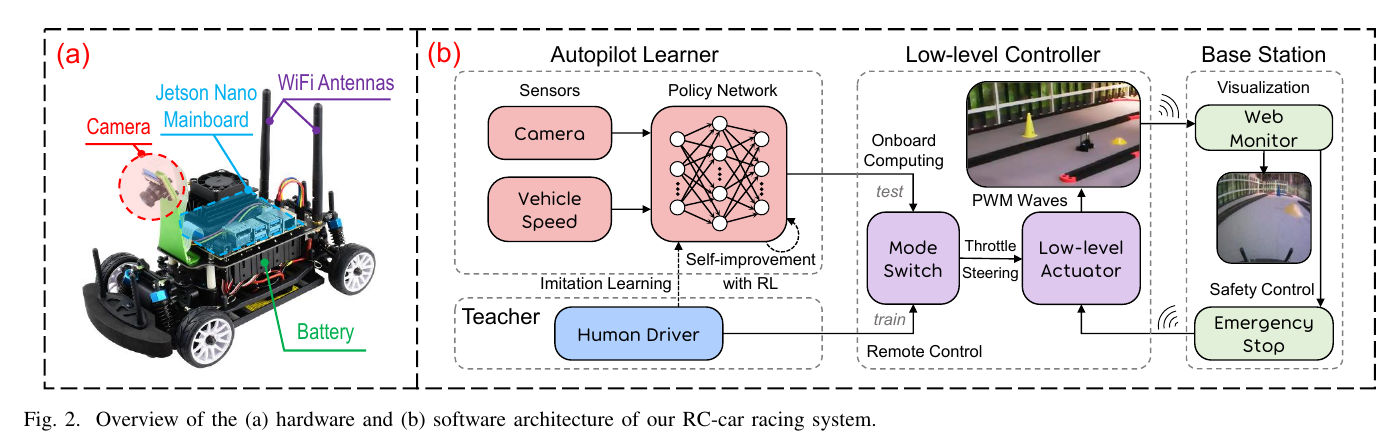
\includegraphics[width=\textwidth]{img/21}\label{fig:21}
    \end{subfigure}
    \begin{subfigure}{0.4\textwidth}
        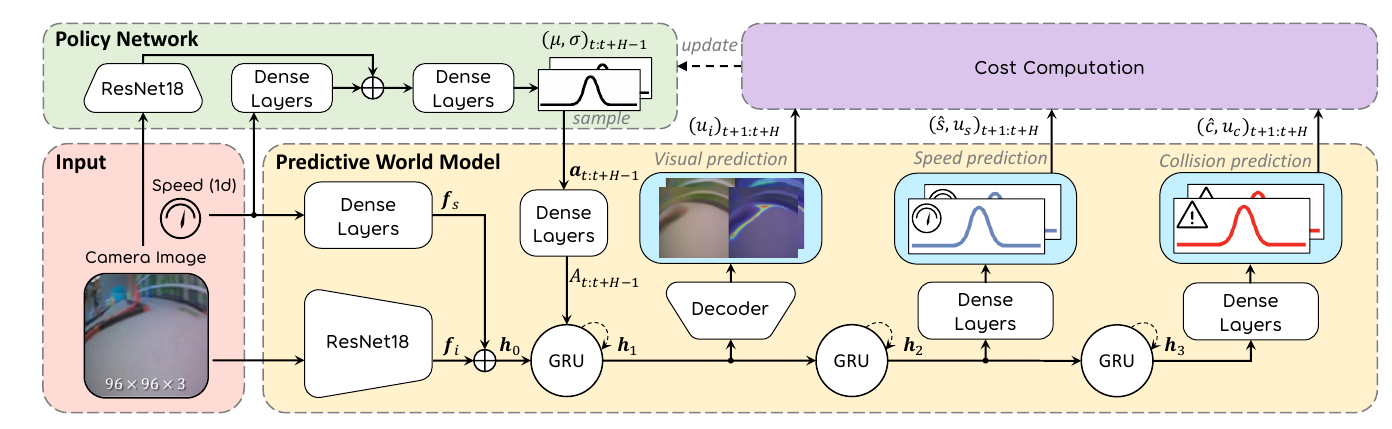
\includegraphics[width=\textwidth]{img/22}\label{fig:22}
    \end{subfigure}
%            \begin{subfigure}
%                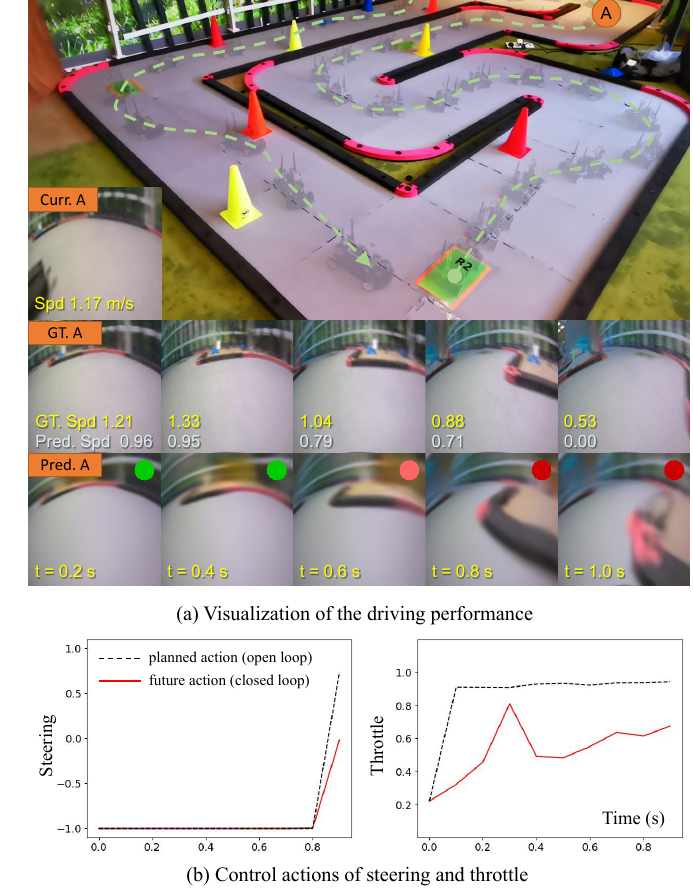
\includegraphics[width=0.2\textwidth]{img/23}\label{fig:23}
%            \end{subfigure}
\end{figure}

\clearpage

\noindent\textbf{Model-based probabilistic collision detection in autonomous driving}~\cite{althoff2009model}
El artículo fue publicado en la revista IEEE Transactions on Intelligent Transportation Systems en 2009 y se centra en la seguridad vial
de los vehículos autónomos en entornos de tráfico complejo.
Su enfoque principal es la detección probabilística de colisiones mediante el análisis y la predicción de la ocupación de la carretera
por parte de otros vehículos.\\
El estudio aborda la incertidumbre inherente en la interacción entre los vehículos autónomos y otros actores del tráfico.
Analiza cómo las mediciones y los posibles comportamientos de estos afectan la predicción de posibles colisiones.
Además, considera las limitaciones en las maniobras de conducción debidas a la geometría de la carretera y la influencia
de estas restricciones en la probabilidad de colisión para trayectorias específicas.\\
Lo más destacado de este enfoque es su eficiencia. La mayor parte de los cálculos intensivos se llevan a cabo offline,
permitiendo disponer de un algoritmo en línea eficiente para aplicaciones en tiempo real.                                                                           \\
Esto contribuye significativamente a la seguridad vial al proporcionar una herramienta precisa y eficaz para la detección anticipada de
posibles colisiones en entornos de conducción autónoma.                                                            \\
\begin{figure}[!ht]
    \begin{subfigure}{0.4\textwidth}
        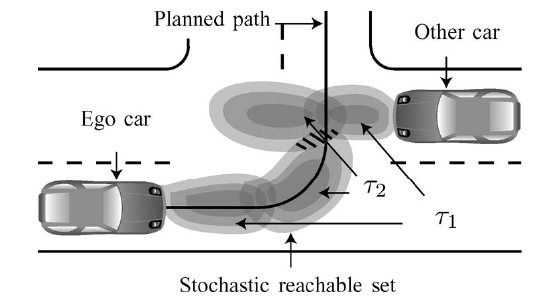
\includegraphics[width=\textwidth]{img/31}\label{fig:31}
    \end{subfigure}
    \begin{subfigure}{0.4\textwidth}
        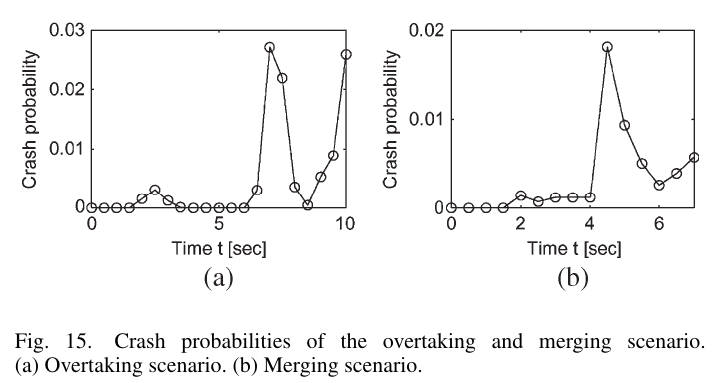
\includegraphics[width=\textwidth]{img/35}\label{fig:35}
    \end{subfigure}
%            \begin{subfigure}
%                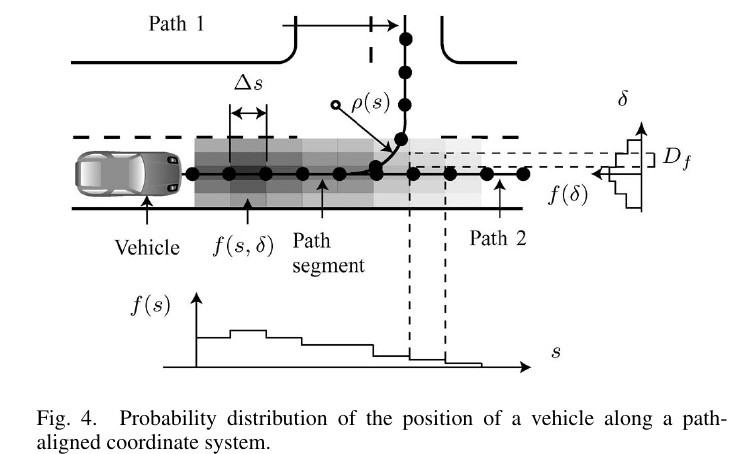
\includegraphics[width=0.5\textwidth]{img/32}\label{fig:32}
%            \end{subfigure}
    \vspace{2cm}
    \begin{subfigure}{0.4\textwidth}
        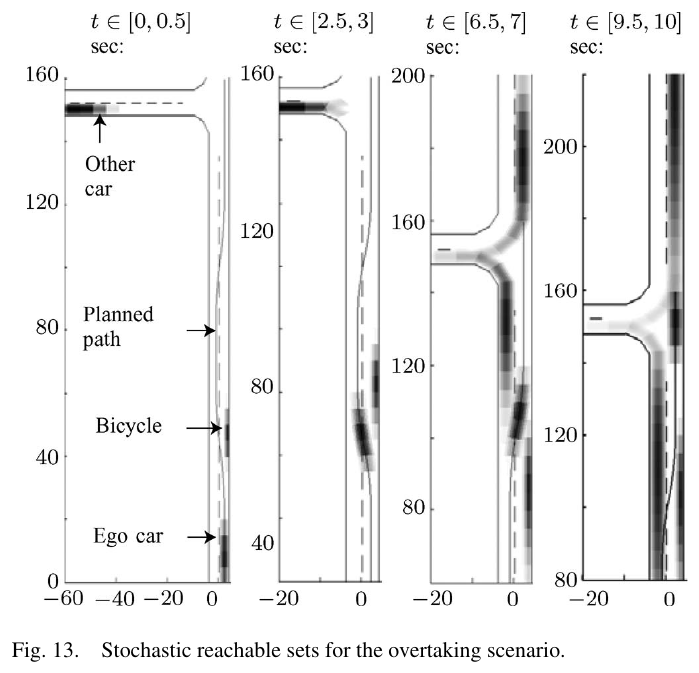
\includegraphics[width=\textwidth]{img/33}\label{fig:33}
    \end{subfigure}
    \begin{subfigure}{0.4\textwidth}
        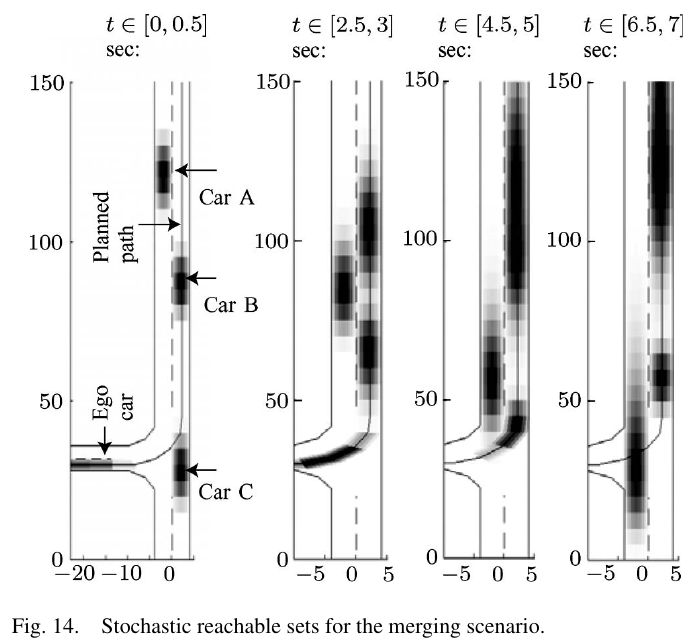
\includegraphics[width=\textwidth]{img/34}\label{fig:34}
    \end{subfigure}

\end{figure}
\clearpage

\noindent\textbf{Vision-based autonomous vehicle systems based on deep learning: A systematic literature review}~\cite{pavel2022vision}
El artículo fue publicado en la revista Applied Science en 2022 y presenta una revisión sistemática de la literatura sobre el empleo
de técnicas de aprendizaje profundo en los sistemas
de vehículos autónomos a lo largo de la última década.                                                                    \\Esta revisión se divide en varios módulos que abarcan distintos aspectos,
desde el análisis de percepción y la toma de decisiones hasta el control, la planificación de trayectorias
y la visualización en sistemas de realidad aumentada tipo HUD.                                                                                                                   \\
Se examinan investigaciones llevadas a cabo entre 2011 y 2021 que se enfocan en la utilización de cámaras RGB como sensores principales
en estos sistemas. Se otorga especial atención a los resultados finales, destacando la visualización en sistemas de realidad aumentada
basados en HUD.                                                                                                      \\Esto incluye advertencias tempranas, marcadores en la carretera para mejorar la navegación y la seguridad, superposición
de información en vehículos y peatones en condiciones visuales extremas para reducir colisiones.
La revisión subraya los métodos actuales de aprendizaje profundo que se basan únicamente en la visión de cámaras RGB, prescindiendo de la
compleja fusión de sensores.                                                                     \\Se espera que este enfoque allane el camino para el desarrollo ágil de sistemas de vehículos autónomos,
siendo prácticos, eficientes y seguros en términos de costos.                                                               \\
\begin{figure}[!ht]
    \centering
    \begin{subfigure}{\textwidth}
        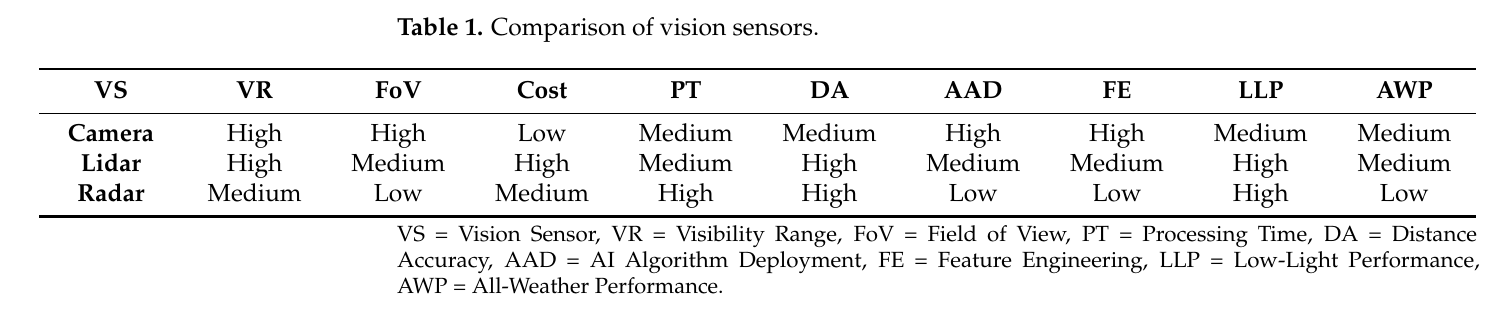
\includegraphics[width=1\textwidth]{img/71}\label{fig:71}
    \end{subfigure}
%            \begin{subfigure}
%                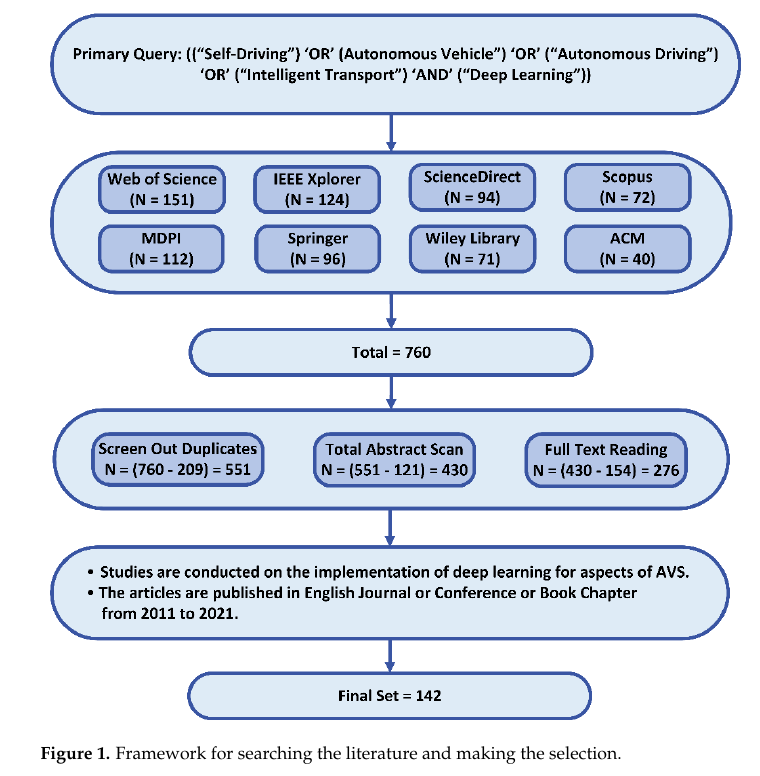
\includegraphics[width=0.5\textwidth]{img/72}\label{fig:72}
%            \end{subfigure}
    \begin{subfigure}{0.4\textwidth}
        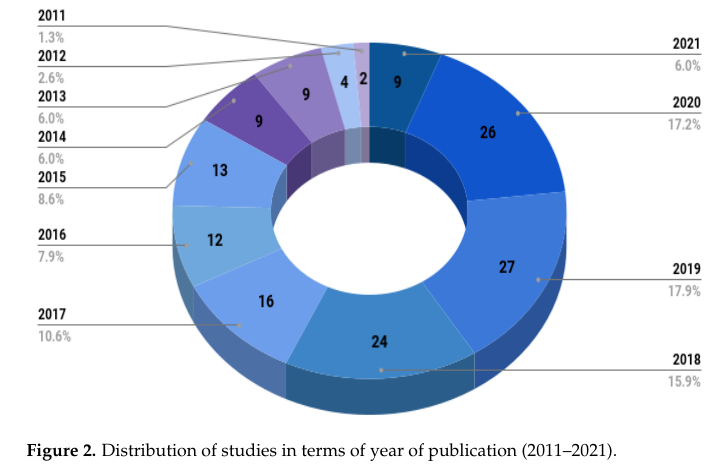
\includegraphics[width=\textwidth]{img/73}\label{fig:73}
    \end{subfigure}
    \begin{subfigure}{0.4\textwidth}
        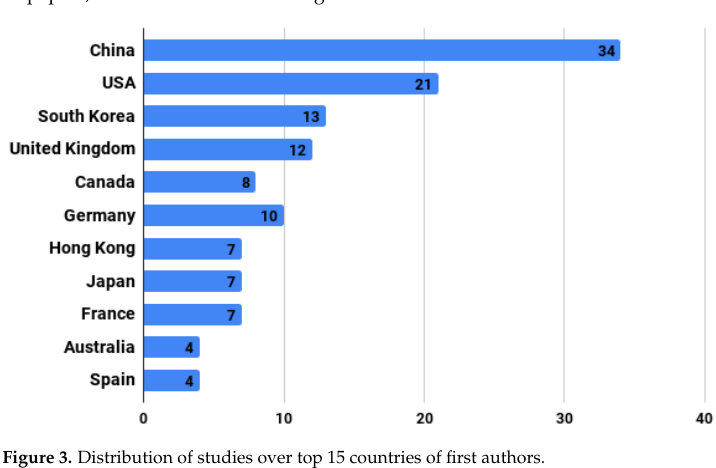
\includegraphics[width=\textwidth]{img/74}\label{fig:74}
    \end{subfigure}
\end{figure}
\clearpage

\noindent\textbf{A cost-effective computer vision-based vehicle detection system}~\cite{alam2022cost}
El artículo fue publicado en la revista Concurrent Engineering en 2022 y se enfoca en la detección de vehículos.
\\Destaca la importancia crítica del procesamiento rápido y la detección precisa de vehículos dentro de un sistema autónomo de detección.
\\Presenta un sistema de detección de vehículos basado en visión por computadora que utiliza un algoritmo de Gentle Adaptive Boosting
con características tipo Haar para generar hipótesis de vehículos de manera eficiente.
Para abordar los errores potenciales, propone el uso de un algoritmo de Máquinas de Vectores de Soporte (SVM) entrenado con características
del histograma de gradientes orientados (HOG) para filtrar las hipótesis falsas.
\\El descriptor HOG se centra en la forma y contornos de los vehículos, mejorando la precisión de la detección.
La combinación de características tipo Haar y HOG permite cumplir los objetivos de detección en la conducción autónoma.
\\El rendimiento del sistema propuesto se evalúa con imágenes capturadas durante el día y la noche y se compara con tres detectores
de vehículos existentes. Los resultados muestran una precisión promedio del 0.97 para imágenes capturadas durante el día
y del 0.94 para imágenes nocturnas.                                                                                               \\Además, se destaca que el sistema propuesto requiere aproximadamente 15 veces menos tiempo
de entrenamiento en comparación con las técnicas existentes, utilizando la misma cantidad de datos de imágenes y la misma unidad
de procesamiento central (CPU). Esto demuestra una mejora significativa en la eficiencia del sistema propuesto en términos de tiempo de entrenamiento.
\begin{figure}[!ht]
\centering
%            \begin{subfigure}
%                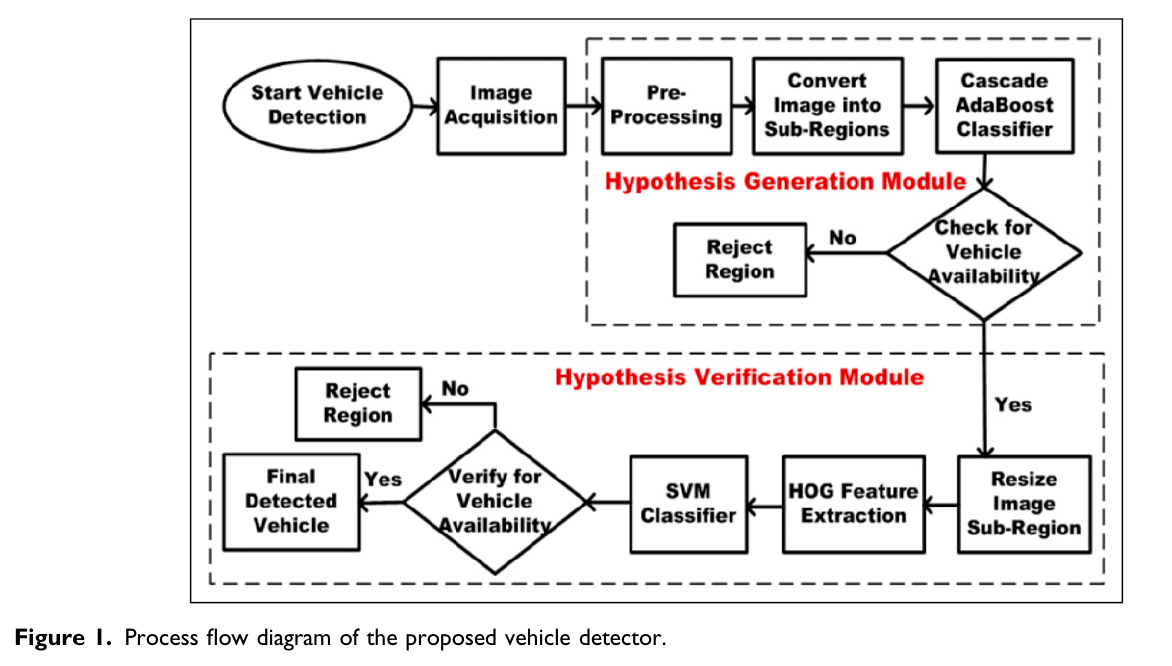
\includegraphics[width=0.6\textwidth]{img/81}\label{fig:81}
%            \end{subfigure}
%            \begin{subfigure}
%                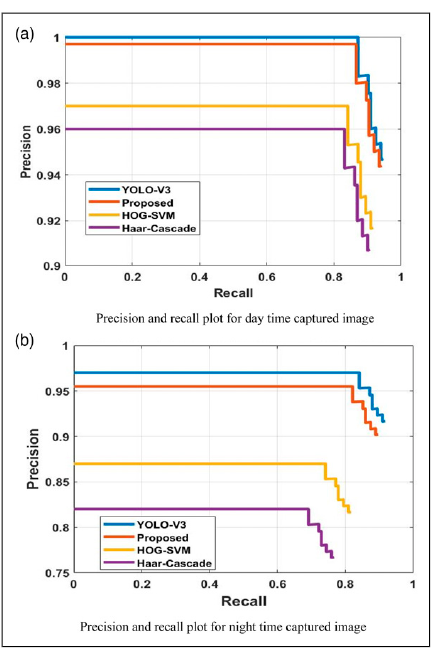
\includegraphics[width=0.5\textwidth]{img/86}\label{fig:82}
%            \end{subfigure}
    \begin{subfigure}{0.4\textwidth}
        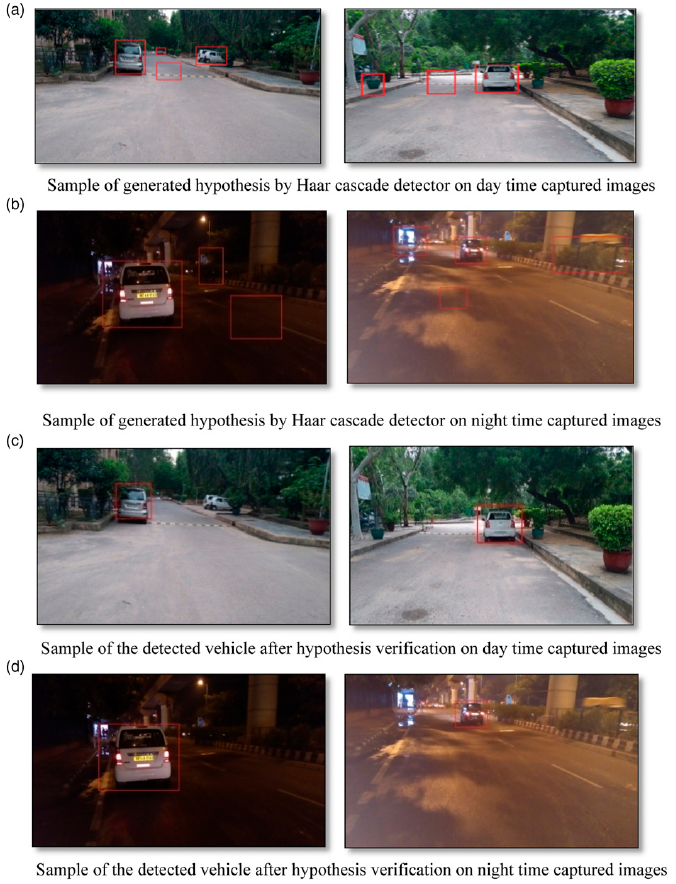
\includegraphics[width=\textwidth]{img/84}\label{fig:84}
    \end{subfigure}
    \begin{subfigure}{0.4\textwidth}
        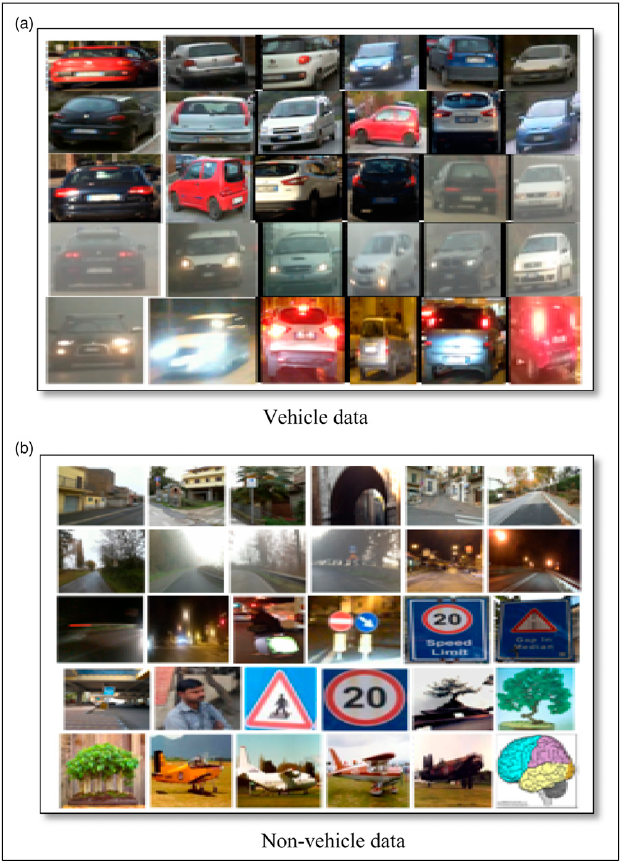
\includegraphics[width=\textwidth]{img/82}\label{fig:86}
    \end{subfigure}
\end{figure}
\clearpage


% \subsection{Tabla comparativa}
% \begin{center}
    \resizebox{\textwidth}{!}{
        \begin{tabular}{|p{5cm}|p{2cm}|p{2cm}|p{2cm}|p{2cm}|p{2cm}|p{2cm}|}
            \hline
            \textbf{Características}
            & \textbf{Propia}
            & \textbf{Autonomous Driving Architectures \cite{bachute2021autonomous}}
            & \textbf{Vision-based Autonomous Car Racing \cite{cai2021vision}}
            & \textbf{Model-based Probabilistic Collision Detection \cite{althoff2009model}}
            & \textbf{Vision-based Autonomous Vehicle Systems \cite{pavel2022vision}}
            & \textbf{Cost-effective Vehicle Detection System \cite{alam2022cost}} \\
            \hline
            Uso de algoritmos de Aprendizaje Automático y Aprendizaje Profundo & X & X &   &   & X &   \\
            \hline
            Enfoque en la conducción autónoma                                  & X & X & X & X & X & X \\
            \hline
            Ventajas de la conducción autónoma                                 & X & X &   &   &   &   \\
            \hline
            Complejidad de los sistemas de conducción autónoma                 &   & X &   &   &   &   \\
            \hline
            Análisis de tareas en la conducción autónoma                       & X & X &   &   &   &   \\
            \hline
            Evaluación y comparación de algoritmos                             &   & X & X &   &   &   \\
            \hline
            Predicción estocástica de ocupación de la carretera                &   &   &   & X &   &   \\
            \hline
            Eficiencia en cálculos intensivos                                  &   &   & X & X &   &   \\
            \hline
            Utilización de cámaras RGB como sensores principales               & X &   & X &   & X &   \\
            \hline
            Detección de vehículos en conducción autónoma                      & X &   &   &   &   & X \\
            \hline
        \end{tabular}
    }
\end{center}

% Capítulo 2: Marco teórico
\clearpage
\chapter{Marco teórico}\label{chap:marco-teorico}
Este capítulo reúne los fundamentos teóricos y computacionales necesarios para comprender la metodología propuesta. Se inicia con la formación de imagen y el modelo de cámara pin-hole, explicando de manera intuitiva la proyección de puntos y líneas, así como la representación homogénea para operaciones geométricas (Sección \ref{subsec:camera}).

A continuación, se abordan las herramientas matemáticas para describir y manipular líneas y puntos en el plano imagen, incluyendo la obtención de líneas a partir de puntos, intersección de líneas, y el ajuste óptimo mediante formulaciones basadas en el espacio nulo (Sección \ref{subsec:lines-points}).

Se presentan las homografías para el plano del suelo (Sección \ref{subsec:homografias}), y las técnicas de detección de bordes y líneas empleadas, en particular el método de Canny y la transformada de Hough (Sección \ref{sec:canny-hough}).

La sección central describe el algoritmo RANSAC para el ajuste robusto de modelos en presencia de outliers, detallando su funcionamiento y parámetros clave según la referencia clásica de Fischler y Bolles y la exposición de Hartley \& Zisserman (Sección \ref{sec:ransac-teorico}).

Finalmente, se establecen las convenciones de marcos de referencia y representación de la pose, y se describen las plataformas y bibliotecas utilizadas, como CARLA y OpenCV (Sección \ref{sec:plataformas}).


\section{Fundamentos de visión por computadora}\label{sec:vision}
En esta sección se resumen los fundamentos teóricos necesarios para el resto del trabajo. Se presentan el modelo de cámara, homografías para el plano del suelo y los operadores de detección de bordes y líneas, así como la notación homogénea para rectas y el concepto de puntos de fuga.

\subsection{Modelo de cámara \emph{pin-hole} y calibración}\label{subsec:camera}

El modelo pin-hole es una aproximación matemática que describe cómo se forma una imagen
en una cámara. Como se muestra en la Fig.~\ref{fig:pinhole-model}, este modelo representa
la cámara como una caja con un pequeño orificio (\emph{pin-hole}) por donde pasa la luz.

\begin{figure}[!ht]
	\centering
	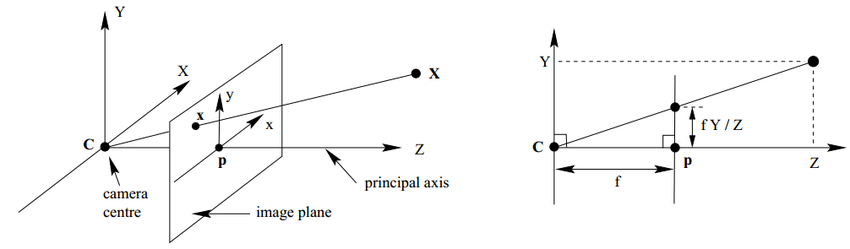
\includegraphics[width=0.99\textwidth]{img/2-mt/pinhole.png}
	\caption{Geometría del modelo de cámara pin-hole. (Imagen de \cite{hartley2003multiple}).}
	\label{fig:pinhole-model}
\end{figure}


En este modelo, un punto tridimensional \(\mathbf{X}\) del mundo se proyecta a través
del centro óptico \(\mathbf{C}\) hacia el plano de imagen, generando el punto bidimensional
\(\mathbf{x}\) en la imagen. Esta proyección es una transformación geométrica que preserva
las líneas rectas pero no las distancias ni los ángulos.


Para aplicaciones prácticas, es necesario conocer los parámetros internos de la cámara
a través del proceso calibración (calibración intrínseca). Esta calibración estima
una matriz de cámara que contiene parámetros como la distancia focal,
el punto principal y el factor de aspecto, así como coeficientes de distorsión.


Con estos parámetros, es posible normalizar las coordenadas de la imagen,
es decir, corregir las distorsiones y convertir píxeles a coordenadas métricas normalizadas.
Esto permite realizar mediciones geométricas más precisas y aplicar algoritmos
de visión por computadora con menor error \cite{hartley2003multiple}.

\subsection{Líneas y puntos en el modelo \emph{pin-hole}}\label{subsec:lines-points}

En el modelo pin-hole, tanto los puntos como las líneas pueden representarse de forma cartesiana u homogénea. La representación homogénea ofrece ventajas computacionales importantes para operaciones geométricas como intersecciones y ajustes de múltiples elementos.

\subsubsection{Representación de puntos}
Un punto en la imagen puede expresarse en coordenadas cartesianas como $(x,y)$ o en coordenadas homogéneas como $\mathbf{x}=[x,y,w]^\top$\footnote{Usualmente para convertir una coordenada cartesiana a homogenea se define $w=1$, aunque cualquier valor diferentes de $0$ puede usarse, si se usa de manera consistente.}. La representación homogénea permite trabajar con transformaciones proyectivas de forma más elegante y manejar puntos en el infinito de manera consistente.

\subsubsection{Representación de líneas}

Una línea en la imagen se representa en coordenadas homogéneas como $\ell=[A,B,C]^\top$, donde $A$, $B$ y $C$ son los parámetros de la ecuación cartesiana de la línea:
\begin{equation}
	Ax + By + C = 0
\end{equation}

\subsubsection{Relación entre líneas y puntos}
Un punto homogéneo $\mathbf{x}$ pertenece a una línea $\ell$ si y solo si:
\begin{equation}
	\ell^\top\mathbf{x} = 0
\end{equation}
Esta relación fundamental permite verificar incidencia y realizar operaciones geométricas de forma algebraica.

\subsubsection{Línea a partir de dos puntos cartesianos}\label{subsec:line-from-points}

Dados dos puntos cartesianos $(x_1,y_1)$ y $(x_2,y_2)$, la línea que los contiene se obtiene resolviendo el sistema:
\begin{equation}
	\begin{bmatrix}x_1&y_1&1\\x_2&y_2&1\end{bmatrix}\begin{bmatrix}A\\B\\C\end{bmatrix} = \mathbf{0}
\end{equation}
La solución $\ell=[A,B,C]^\top$ se encuentra calculando el espacio nulo de la matriz $\mathbf{M}$. Existen varias formas de obtener este espacio nulo, entre ellas una posible forma de hacerlo de manera simple es mediante descomposición en valores singulares (SVD) para mayor robustez numérica \cite{golub2013matrix}.

\subsubsection{Línea a partir de dos puntos homogéneos}

Si los puntos están en coordenadas homogéneas $\mathbf{x}_1$ y $\mathbf{x}_2$, la línea se calcula directamente con el producto cruz:
\begin{equation}
	\ell = \mathbf{x}_1 \times \mathbf{x}_2
\end{equation}

\subsubsection{Intersección de dos líneas}
Dadas dos líneas homogéneas $\ell_1$ y $\ell_2$, su punto de intersección se obtiene mediante:
\begin{equation}
	\mathbf{x} = \ell_1 \times \ell_2
\end{equation}

      
Sea $\mathbf{x}=[x_1,x_2,x_3]^\top$ una coordenada homogenea. Si $x_3 \neq 0$, el punto es finito y se deshomogeneiza como $(w\frac{x_1}{x_3}, w\frac{x_2}{x_3})$ . Valores $x_3 \approx 0$ indican líneas prácticamente paralelas con intersección en el infinito \cite{hartley2003multiple}.

\subsubsection{Ajuste a múltiples elementos} \label{sec:ajuste-multiples-elementos}

Para encontrar la mejor línea que pase por múltiples puntos, o el mejor punto de intersección de múltiples líneas, la solución óptima está dada por el eigenvector asociado al eigenvalor más pequeño de la matriz $\mathbf{M}$ \cite{kanatani1998statistical} que se define a continuación:
\begin{equation}
	\mathbf{M} = \sum_{i=1}^{n} w_i \mathbf{v}_i \mathbf{v}_i^\top
\end{equation}
donde $\mathbf{v}_i$ representa:
\begin{itemize}
	\item puntos homogéneos $\mathbf{x}_i$ para encontrar la línea que mejor se ajuste a los puntos
	\item líneas homogéneas $\ell_i$ para encontrar el punto de intersección de las líneas
\end{itemize} y  $w_i$ es una ponderación tal que:
\[
\sum_{i=1}^{n} w_i = 1.
\]

\subsection{Homografías en el plano del suelo}\label{subsec:homografias}

Cuando los puntos pertenecen a un mismo plano (\emph{e.g.}, el suelo),
la relación entre sus proyecciones en  dos vistas o entre el plano del
mundo   y    la   imagen   puede   modelarse    con   una   homografía
\(\mathbf{H}\in\mathbb{R}^{3\times3}\)      definida     a      escala
\cite{hartley2003multiple}. Esta  matriz permite  mapear cuadriláteros
en la imagen a cuadrados canónicos, facilitando medir y extrapolar una
retícula en la imagen.

\subsection{Bordes y líneas: Canny y Hough}\label{sec:canny-hough}

La extracción de bordes con Canny proporciona contornos estables frente a ruido mediante suavizado, gradiente y supresión no máxima \cite{canny1986edge}. La transformada de Hough detecta lineas rectas parametrizando la ecuación\[\rho=x\cos{\theta}+y\sin{\theta}\] donde $\rho$ es la distancia mínima de la recta al origen y $\theta$ es el ángulo de la normal a la recta\cite{DudaEtAl1972} {\bfseries TODO: Añadir grafica mostrando los parametros rho y theta, y mostrando el resultado de aplicar Canny a una imagen}. Estas dos herramientas permiten obtener segmentos candidatos a las marcas viales de la retícula.

\subsection{Intersecciones de líneas y \emph{clustering}}\label{sec:intersections-clustering}

En escenas urbanas muchas rectas convergen hacia uno o varios puntos de fuga. Por tanto, las
intersecciones finitas tienden a concentrarse en vecindades cercanas a la línea del horizonte. Un filtrado previo por banda horizontal reduce ruido: se retienen solo las intersecciones con \(y\) dentro de una franja alrededor del horizonte estimado (véase sección~\ref{sec:vanishing-points}).


Para consolidar evidencia y atenuar datos atípicos, se agrupan las intersecciones relevantes mediante técnicas de \emph{clustering} no supervisado. Una opción práctica es el \emph{Clustering acumulativo} con umbral de distancia para dejar que los datos determinen el número de cúmulos \cite{tan2005introduction}. Los centroides de los cúmulos proporcionan estimaciones iniciales de puntos de fuga\cite{kanatani1998statistical,hartley2003multiple}.


En resumen, el proceso básico para encontrar puntos es fuga es el siguiente: (i) estimar rectas, (ii) generar intersecciones por pares, (iii) filtrar por banda cercana al horizonte, (iv) agrupar por proximidad, y (v) usar los centroides de cúmulos como candidatos a puntos de fuga para la separación de haces de líneas.

\subsection{Puntos de fuga}\label{sec:vanishing-points}

Cuando proyectamos una escena del mundo real en tres dimensiones sobre un plano bidimensional,
como la película o el sensor de una cámara, se produce una transformación en la imagen.
Esta transformación, conocida como transformación proyectiva, provoca que las líneas paralelas en el mundo real,
al proyectarse en el plano de la cámara, se intersecten en un punto denominado punto de fuga.
La Fig.~\ref{fig:distorion-teo} ilustra el fenómeno de paralelismo en 3D y su proyección en 2D.

\begin{figure}[!ht]
	\centering
	\begin{subfigure}{0.4\textwidth}
		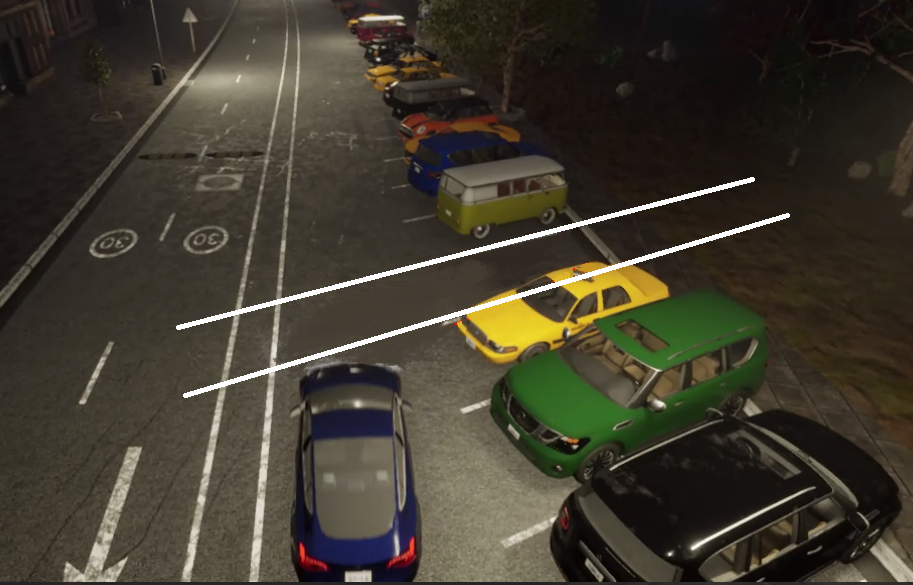
\includegraphics[width=\textwidth]{img/reticule/paralel_lines}
		\caption{Ejemplo de líneas paralelas en un escenario real en tres dimensiones.}
	\end{subfigure}
	\begin{subfigure}{0.4\textwidth}
		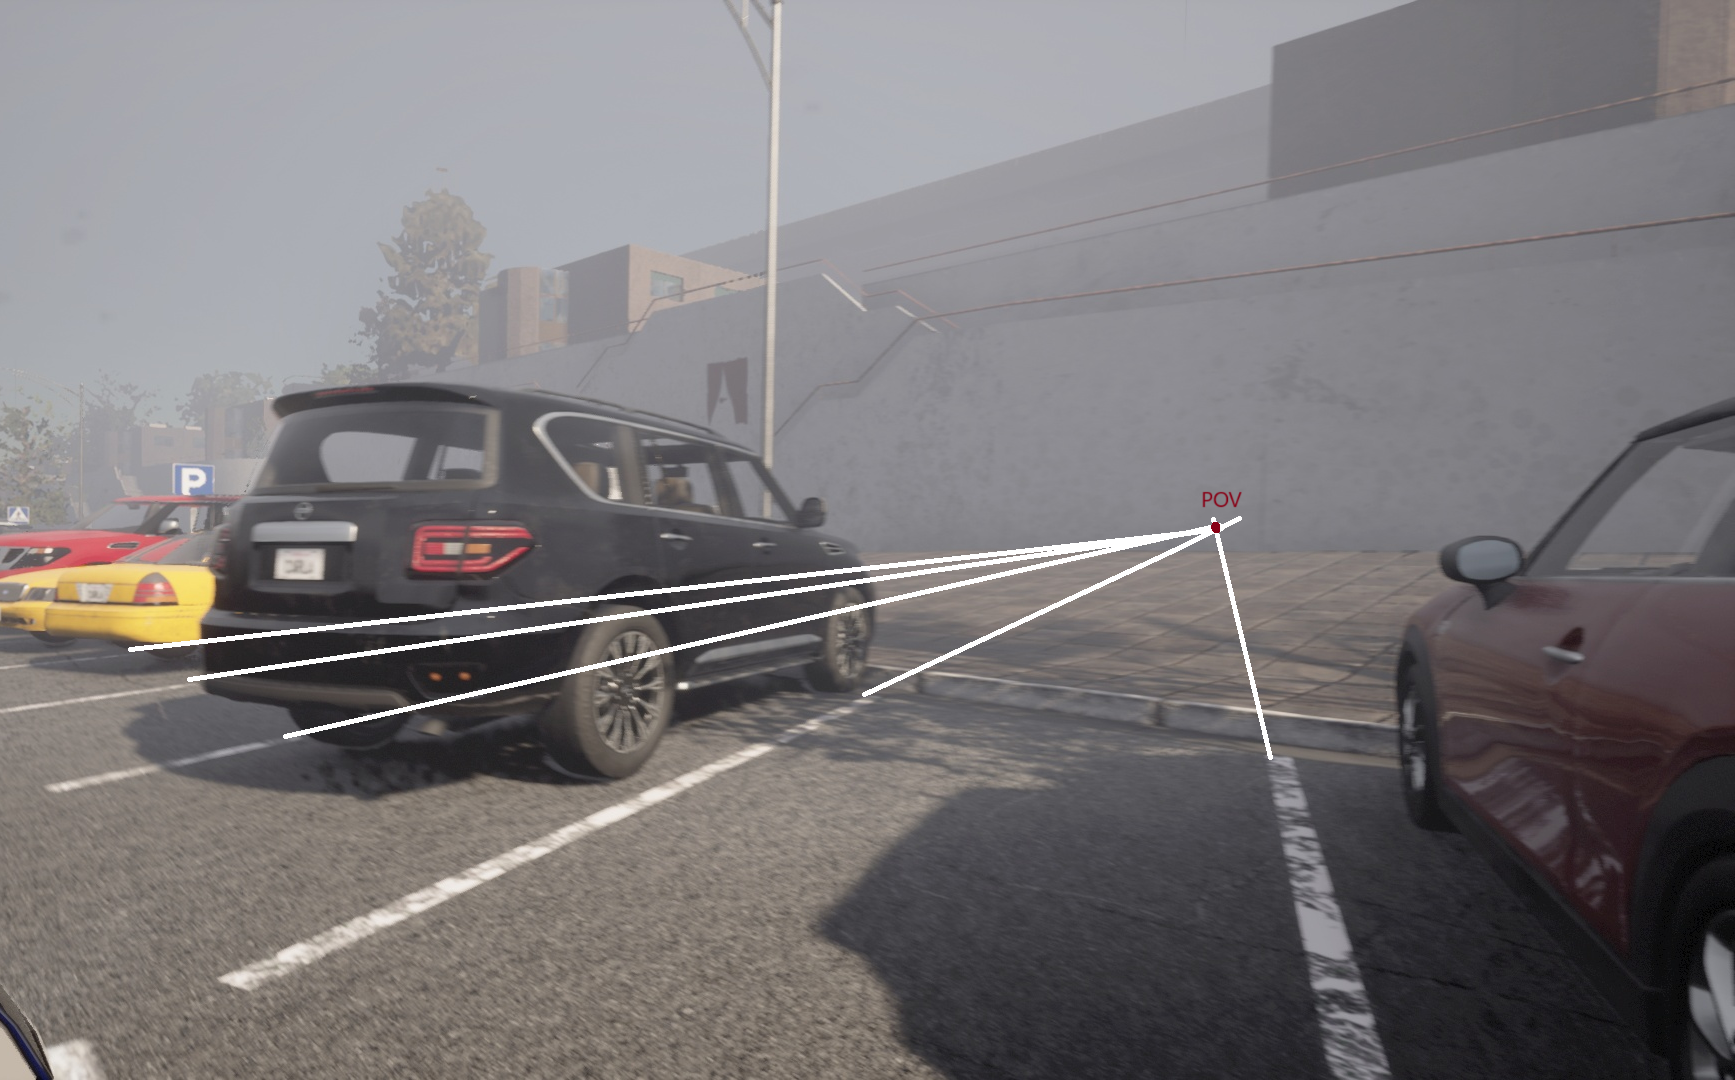
\includegraphics[width=\textwidth]{img/reticule/pov}
		\caption{Proyección de líneas paralelas en el plano de la cámara.}
	\end{subfigure}
	\caption{Paralelismo en 3D y su proyección al plano de imagen.}
	\label{fig:distorion-teo}
\end{figure}


Estimar puntos de fuga con múltiples líneas y criterios robustos reduce la sensibilidad a ruido y oclusiones
\cite{hartley2003multiple,kanatani1998statistical}. En este trabajo se emplean dos puntos de fuga para separar
las marcas de la retícula en dos conjuntos según su punto de fuga, coherentes con la geometría del estacionamiento.


\section{RANSAC para homografías basadas en líneas}\label{sec:ransac-teorico}
\noindent
RANSAC (Random Sample Consensus) es un paradigma de estimación robusta de modelos que alterna 
muestreos aleatorios mínimos con una evaluación de consenso (inliers) para encontrar hipótesis 
consistentes aun en presencia de una proporción elevada de datos atípicos. 
En cada iteración se selecciona un subconjunto mínimo de observaciones, se ajusta un modelo candidato 
y se mide cuántas observaciones concuerdan con él dentro de una tolerancia; tras múltiples iteraciones, 
se elige la hipótesis con mayor soporte y, opcionalmente, se refina con los inliers. 
Esta estrategia, ampliamente utilizada en visión por computadora y cartografía automatizada, 
fue introducida por Fischler y Bolles \cite{fischler1981ransac}.

\noindent
Beneficios clave del enfoque RANSAC:
\begin{itemize}
	\item Tolerancia a outliers y ruido: puede recuperar el modelo correcto aunque una parte sustancial de las observaciones sea espuria u ocluida.
	\item Flexibilidad de modelo: se aplica a múltiples familias (rectas, homografías, transformaciones, etc.).
	\item Sencillez operativa: alterna muestreo mínimo, ajuste y conteo de consenso.
\end{itemize}

\noindent
Variación propuesta en este trabajo. 
Como se explicará con más detalle en la Sección \ref{sec:metodo-ransac}, 
en esta investigación adaptamos RANSAC para estimar una homografía que alinee una retícula ideal 
con las líneas de los cajones de estacionamiento observadas en la imagen. 
Bajo las siguientes consideraciones generales: 
(i) se emplean dos puntos de fuga para agrupar las líneas en dos conjuntos según su punto de fuga; 
(ii) la muestra mínima se construye eligiendo dos líneas de cada conjunto (uno por cada punto de fuga) para formar cuatro intersecciones 
que hipotetizan un cajón; y 
(iii) a partir de esas esquinas se estima una homografía y se extiende una retícula \(n\times n\) 
sobre la imagen. Este planteamiento proporciona coherencia geométrica global del patrón 
y permite extrapolar la retícula más allá del campo visible, infiriendo la ubicación de cajones 
en puntos ciegos o parcialmente ocultos, lo cual resulta útil para la planificación 
y el estacionamiento automático.


\section{Aprendizaje por refuerzo}

El aprendizaje por refuerzo (RL, por sus siglas en inglés) constituye un paradigma de la inteligencia artificial
que permite a un agente aprender a tomar decisiones óptimas mediante la interacción con un entorno.
A diferencia del aprendizaje supervisado, donde se dispone de ejemplos etiquetados, o del no supervisado,
que busca patrones ocultos, el aprendizaje por refuerzo se basa en un proceso de prueba y error donde el agente
recibe retroalimentación en forma de recompensas o penalizaciones según las consecuencias de sus acciones.


La IA puede contribuir significativamente a la mejora de los sistemas de asistencia al conductor.
Si una IA aprendiera a estacionar un vehículo en un ambiente controlado, este conocimiento podría
proporcionar información valiosa para automatizar esta tarea compleja. Los algoritmos de aprendizaje
por refuerzo son candidatos naturales para este tipo de problemas secuenciales de toma de decisiones.

\subsection{Componentes fundamentales del aprendizaje por refuerzo}\label{subsec:rl-components}

El framework de aprendizaje por refuerzo se estructura alrededor de la interacción cíclica entre
cuatro elementos principales representados en la figura \ref{fig:rl-cycle}:

\begin{figure}[!ht]
    \centering
    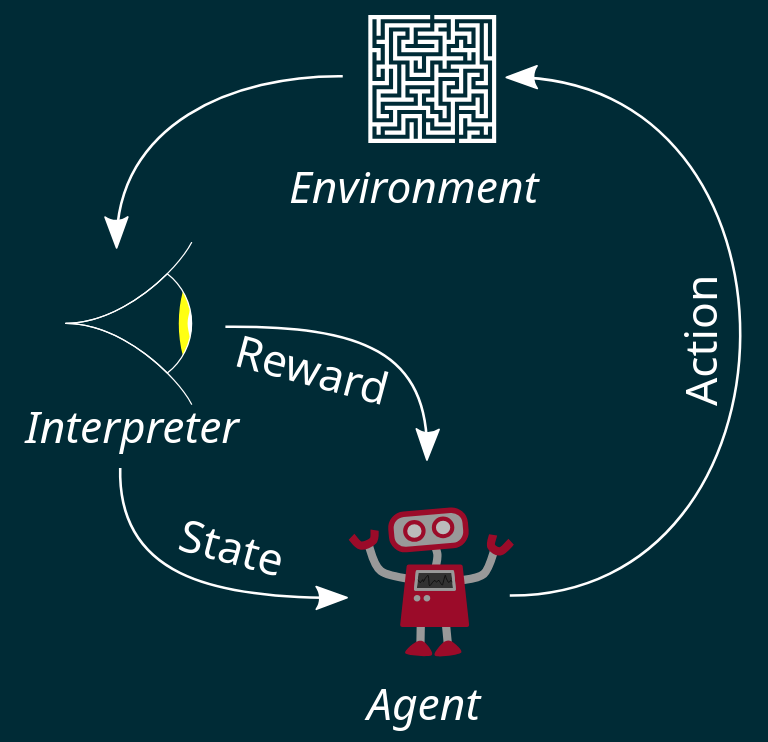
\includegraphics[width=0.5\textwidth]{img/2-mt/RL.png}
    \caption{Ciclo básico del aprendizaje por refuerzo: interacción agente-entorno.}
    \label{fig:rl-cycle}
\end{figure}

\begin{itemize}
    \item \textbf{Agente}: entidad que toma decisiones y ejecuta acciones. En el contexto de estacionamiento automático,
    el agente corresponde al sistema de control del vehículo que decide las maniobras a realizar.
    
    \item \textbf{Entorno}: sistema o mundo en el que opera el agente. Para estacionamiento, incluye
    el espacio físico del estacionamiento, otros vehículos, obstáculos y las leyes físicas que gobiernan
    el movimiento vehicular.
    
    \item \textbf{Estado}: representación de la situación actual del sistema. Típicamente incluye
    información sobre la posición, orientación y velocidad del vehículo, así como la disposición
    del entorno circundante.
    
    \item \textbf{Acción}: decisión o maniobra que el agente puede ejecutar para cambiar el estado
    del entorno. En conducción, las acciones básicas incluyen acelerar, frenar y girar el volante.
    
    \item \textbf{Recompensa}: señal numérica que evalúa qué tan buena o mala fue una acción particular
    en un estado dado. Una función de recompensa bien diseñada guía al agente hacia comportamientos deseables
    (como estacionar correctamente) y penaliza acciones indeseables (como colisiones).
    
    \item \textbf{Política}: estrategia que determina qué acción tomar en cada estado. El objetivo
    del aprendizaje por refuerzo es encontrar una política óptima que maximice la recompensa acumulada.
\end{itemize}

\subsection{Aplicación al estacionamiento automático}\label{subsec:rl-parking}

En el problema de estacionamiento automático, el agente (vehículo) debe aprender a navegar desde
una posición inicial hasta un cajón de estacionamiento objetivo, evitando obstáculos y respetando
las limitaciones físicas del vehículo. El estado puede incluir la pose del vehículo (posición y orientación)
relativa al objetivo, mientras que las acciones corresponden a comandos de aceleración y dirección.


La recompensa típicamente incorpora múltiples criterios: proximidad al objetivo, penalizaciones por colisiones,
suavidad de la trayectoria y cumplimiento de restricciones geométricas del estacionamiento.
Un intérprete basado en sensores (como el sistema de visión desarrollado en este trabajo) proporciona
la información de estado necesaria para que el agente tome decisiones informadas.


Esta aproximación permite que el sistema aprenda estrategias de estacionamiento sin programación explícita
de todas las situaciones posibles, adaptándose a diferentes configuraciones de estacionamiento y
condiciones del entorno a través de la experiencia acumulada durante el entrenamiento.


\section{Plataformas y librerías}\label{sec:plataformas}

La simulación computacional se ha consolidado como una herramienta fundamental
en el desarrollo y validación de sistemas de conducción autónoma.
Permite recrear escenarios complejos y potencialmente peligrosos de manera segura,
flexible y económica, facilitando la experimentación y el análisis de algoritmos
antes de su implementación en vehículos reales. En el contexto de este trabajo,
la simulación resulta especialmente útil para modelar situaciones de estacionamiento
automático, donde la precisión y la seguridad son críticas. A través de la simulación,
es posible ajustar parámetros, evaluar el desempeño de sensores virtuales y analizar el
comportamiento del sistema bajo diferentes condiciones ambientales y de tráfico,
todo ello sin los riesgos y costos asociados a las pruebas físicas.
La simulación puede proporcionar información detallada sobre el vehículo y
su entorno, lo que permite realizar mediciones y análisis exhaustivos de los
datos obtenidos, de manera similar a como se haría en la vida real.

En este trabajo se emplean plataformas y bibliotecas ampliamente adoptadas en visión
por computadora y simulación para vehículos autónomos.
En particular, utilizamos CARLA, un simulador de código abierto que permite recrear entornos urbanos realistas
con agentes dinámicos y sensores virtuales configurables, y OpenCV, una biblioteca de procesamiento
de imágenes que proporciona las operaciones básicas para umbralización, detección de bordes (Canny)
y detección de líneas (Hough), entre otras.

\subsection{CARLA Simulator}\label{sec:carla-teorico}

CARLA (Car Learning to Act) es una plataforma orientada a investigación que facilita la generación de escenas
complejas y controladas, con variabilidad de clima, iluminación y tráfico, y un conjunto de sensores virtuales
(cámaras, LiDAR, radar, GPS) que producen datos cercanos a los de un vehículo real.
Su flexibilidad para instrumentar escenarios y capturar datos reproducibles lo hace idóneo para
experimentación y validación de algoritmos de percepción, localización y control en contextos como el
estacionamiento automático \cite{dosovitskiy2017carla}.
En la Sección \ref{subsec:simulation-design} se detalla el diseño específico del entorno de simulación que
utilizamos, y en la Figura~\ref{fig:carla-simulator-teo} (véase Sección \ref{sec:carla-teorico}) se ilustran ejemplos
de condiciones ambientales configurables en la plataforma.

\begin{figure}[!ht]
	\centering
	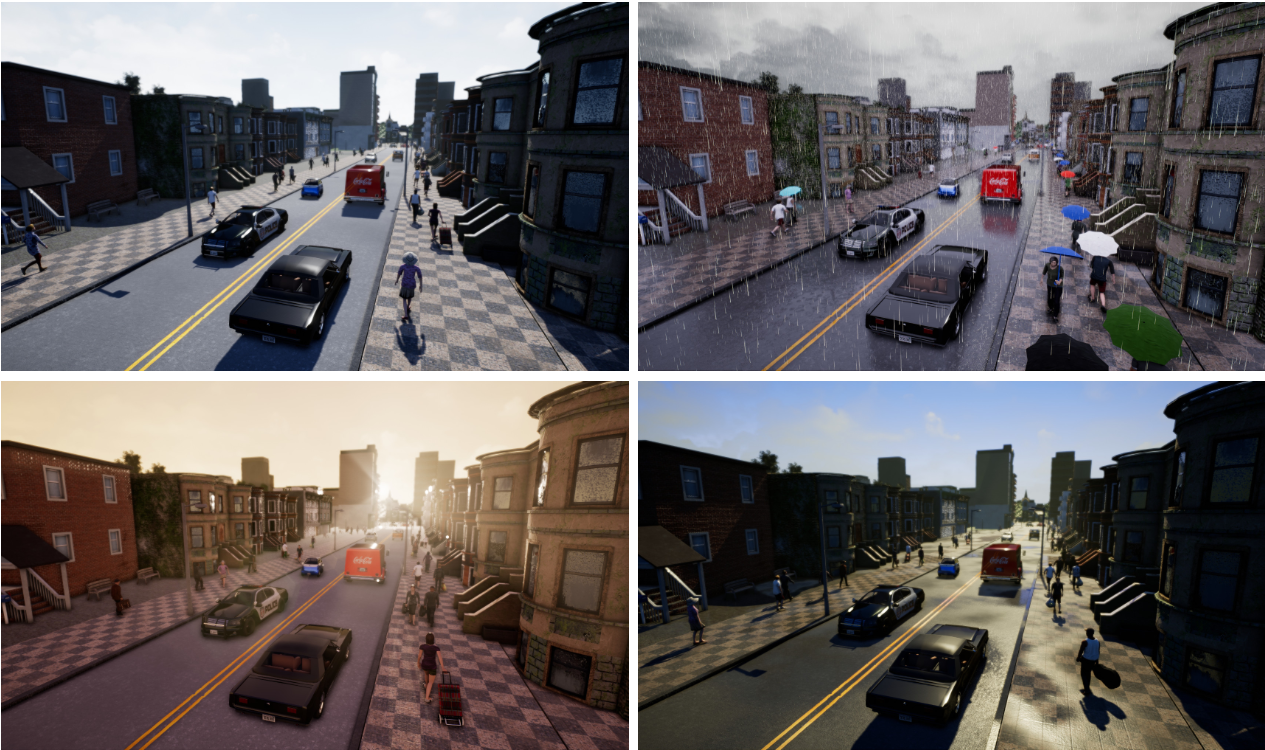
\includegraphics[width=0.8\textwidth]{img/carla_clima_example}
	\caption{Ejemplos de condiciones ambientales configurables en el simulador CARLA.}
	\label{fig:carla-simulator-teo}
\end{figure}

\subsection{OpenCV}

OpenCV proporciona el conjunto de operaciones y estructuras necesarias para el preprocesado de imágenes y la extracción de primitivas geométricas, incluyendo umbralización, Canny y la transformada de Hough, que se emplean en la detección de la retícula de estacionamiento.

\subsection{scikit-learn: \texttt{AgglomerativeClustering}}\label{sec:sklearn-agglomerative}

Para la agrupación de intersecciones utilizamos el algoritmo de \emph{clustering} jerárquico aglomerativo provisto por \texttt{scikit-learn}.
Este enfoque construye una jerarquía de fusiones de abajo hacia arriba, uniendo en cada paso los grupos más próximos según
una métrica de distancia y un criterio de enlace (\texttt{linkage} en \{\texttt{ward}, \texttt{complete}, \texttt{average}, \texttt{single}\}).
El parámetro \texttt{distance\_threshold} permite dejar que el propio algoritmo determine el número de clusters deteniendo
las fusiones cuando la distancia supera un umbral, lo cual resulta práctico en escenas con variabilidad de densidad.
Esta técnica es apropiada para consolidar intersecciones cercanas al horizonte en cúmulos cuya localización (centroide)
sirve de estimación inicial de puntos de fuga \cite{tan2005introduction}.

\subsection{Gymnasium}\label{sec:gymnasium}

Gymnasium es la biblioteca estándar para entornos de aprendizaje por refuerzo que proporciona una interfaz
unificada entre agentes y entornos \cite{towers2024gymnasium}. Sus principales ventajas incluyen:
compatibilidad con múltiples algoritmos de RL, estandarización de espacios de acción y observación,
y un ecosistema extenso de entornos preconfigurados. Los \texttt{Wrappers} permiten modificar el comportamiento
de entornos existentes sin alterar su código base, facilitando adaptaciones como normalización de observaciones,
transformación de espacios de acción, o integración con simuladores externos.

\subsection{Stable-Baselines3}\label{sec:stable-baselines3}

Stable-Baselines3 (SB3) es una biblioteca que implementa algoritmos de aprendizaje por refuerzo de última
generación con código confiable y bien documentado \cite{raffin2021stable}. Incluye algoritmos como
PPO (Proximal Policy Optimization), SAC (Soft Actor-Critic), TD3 (Twin Delayed Deep Deterministic Policy Gradient),
y soporte para técnicas avanzadas como HER (Hindsight Experience Replay). Su diseño modular permite
experimentación rápida con diferentes algoritmos manteniendo consistencia en hiperparámetros y evaluación.

\subsection{Herramienta de experimentación y ajuste de parámetros}\label{sec:experimentation-tool}

Para determinar la configuración óptima de parámetros de la solución propuesta, se desarrolló una aplicación en Python
que carga una secuencia de imágenes de la trayectoria del vehículo en el estacionamiento y, para cada cuadro,
calcula la retícula aplicando los pasos descritos en este trabajo. La herramienta permite visualizar el resultado de cada
etapa y ajustar dinámicamente los parámetros para analizar su impacto en tiempo real.


Parámetros ajustables considerados:
\begin{itemize}
	\item \texttt{threshold\_image}: Umbral de binarización de la imagen.
	\item \texttt{canny\_threshold\_1}: Umbral inferior para Canny.
	\item \texttt{canny\_threshold\_2}: Umbral superior para Canny.
	\item \texttt{hough\_rho}: Resolución de distancia (píxeles) en Hough.
	\item \texttt{hough\_theta}: Resolución angular (radianes) en Hough.
	\item \texttt{hough\_threshold}: Umbral de votos en Hough.
	\item \texttt{hough\_min\_line\_length}: Longitud mínima de segmento.
	\item \texttt{hough\_max\_line\_gap}: Máxima separación para unir segmentos.
	\item \texttt{relevant\_intersections\_horizon\_threshold}: Umbral de cercanía al horizonte.
	\item \texttt{agglomerative\_distance\_threshold}: Distancia máxima para pertenecer al mismo cúmulo.
\end{itemize}


A modo ilustrativo, a continuación  en la figura \ref{fig:experimentationBinary-teo} 
se muestra la herramienta donde se visualizan contornos, líneas detectadas,
intersecciones, intersecciones relevantes, cúmulos y puntos de fuga.

\begin{figure}[!ht]
	% \begin{subfigure}{0.5\textwidth}
	% 	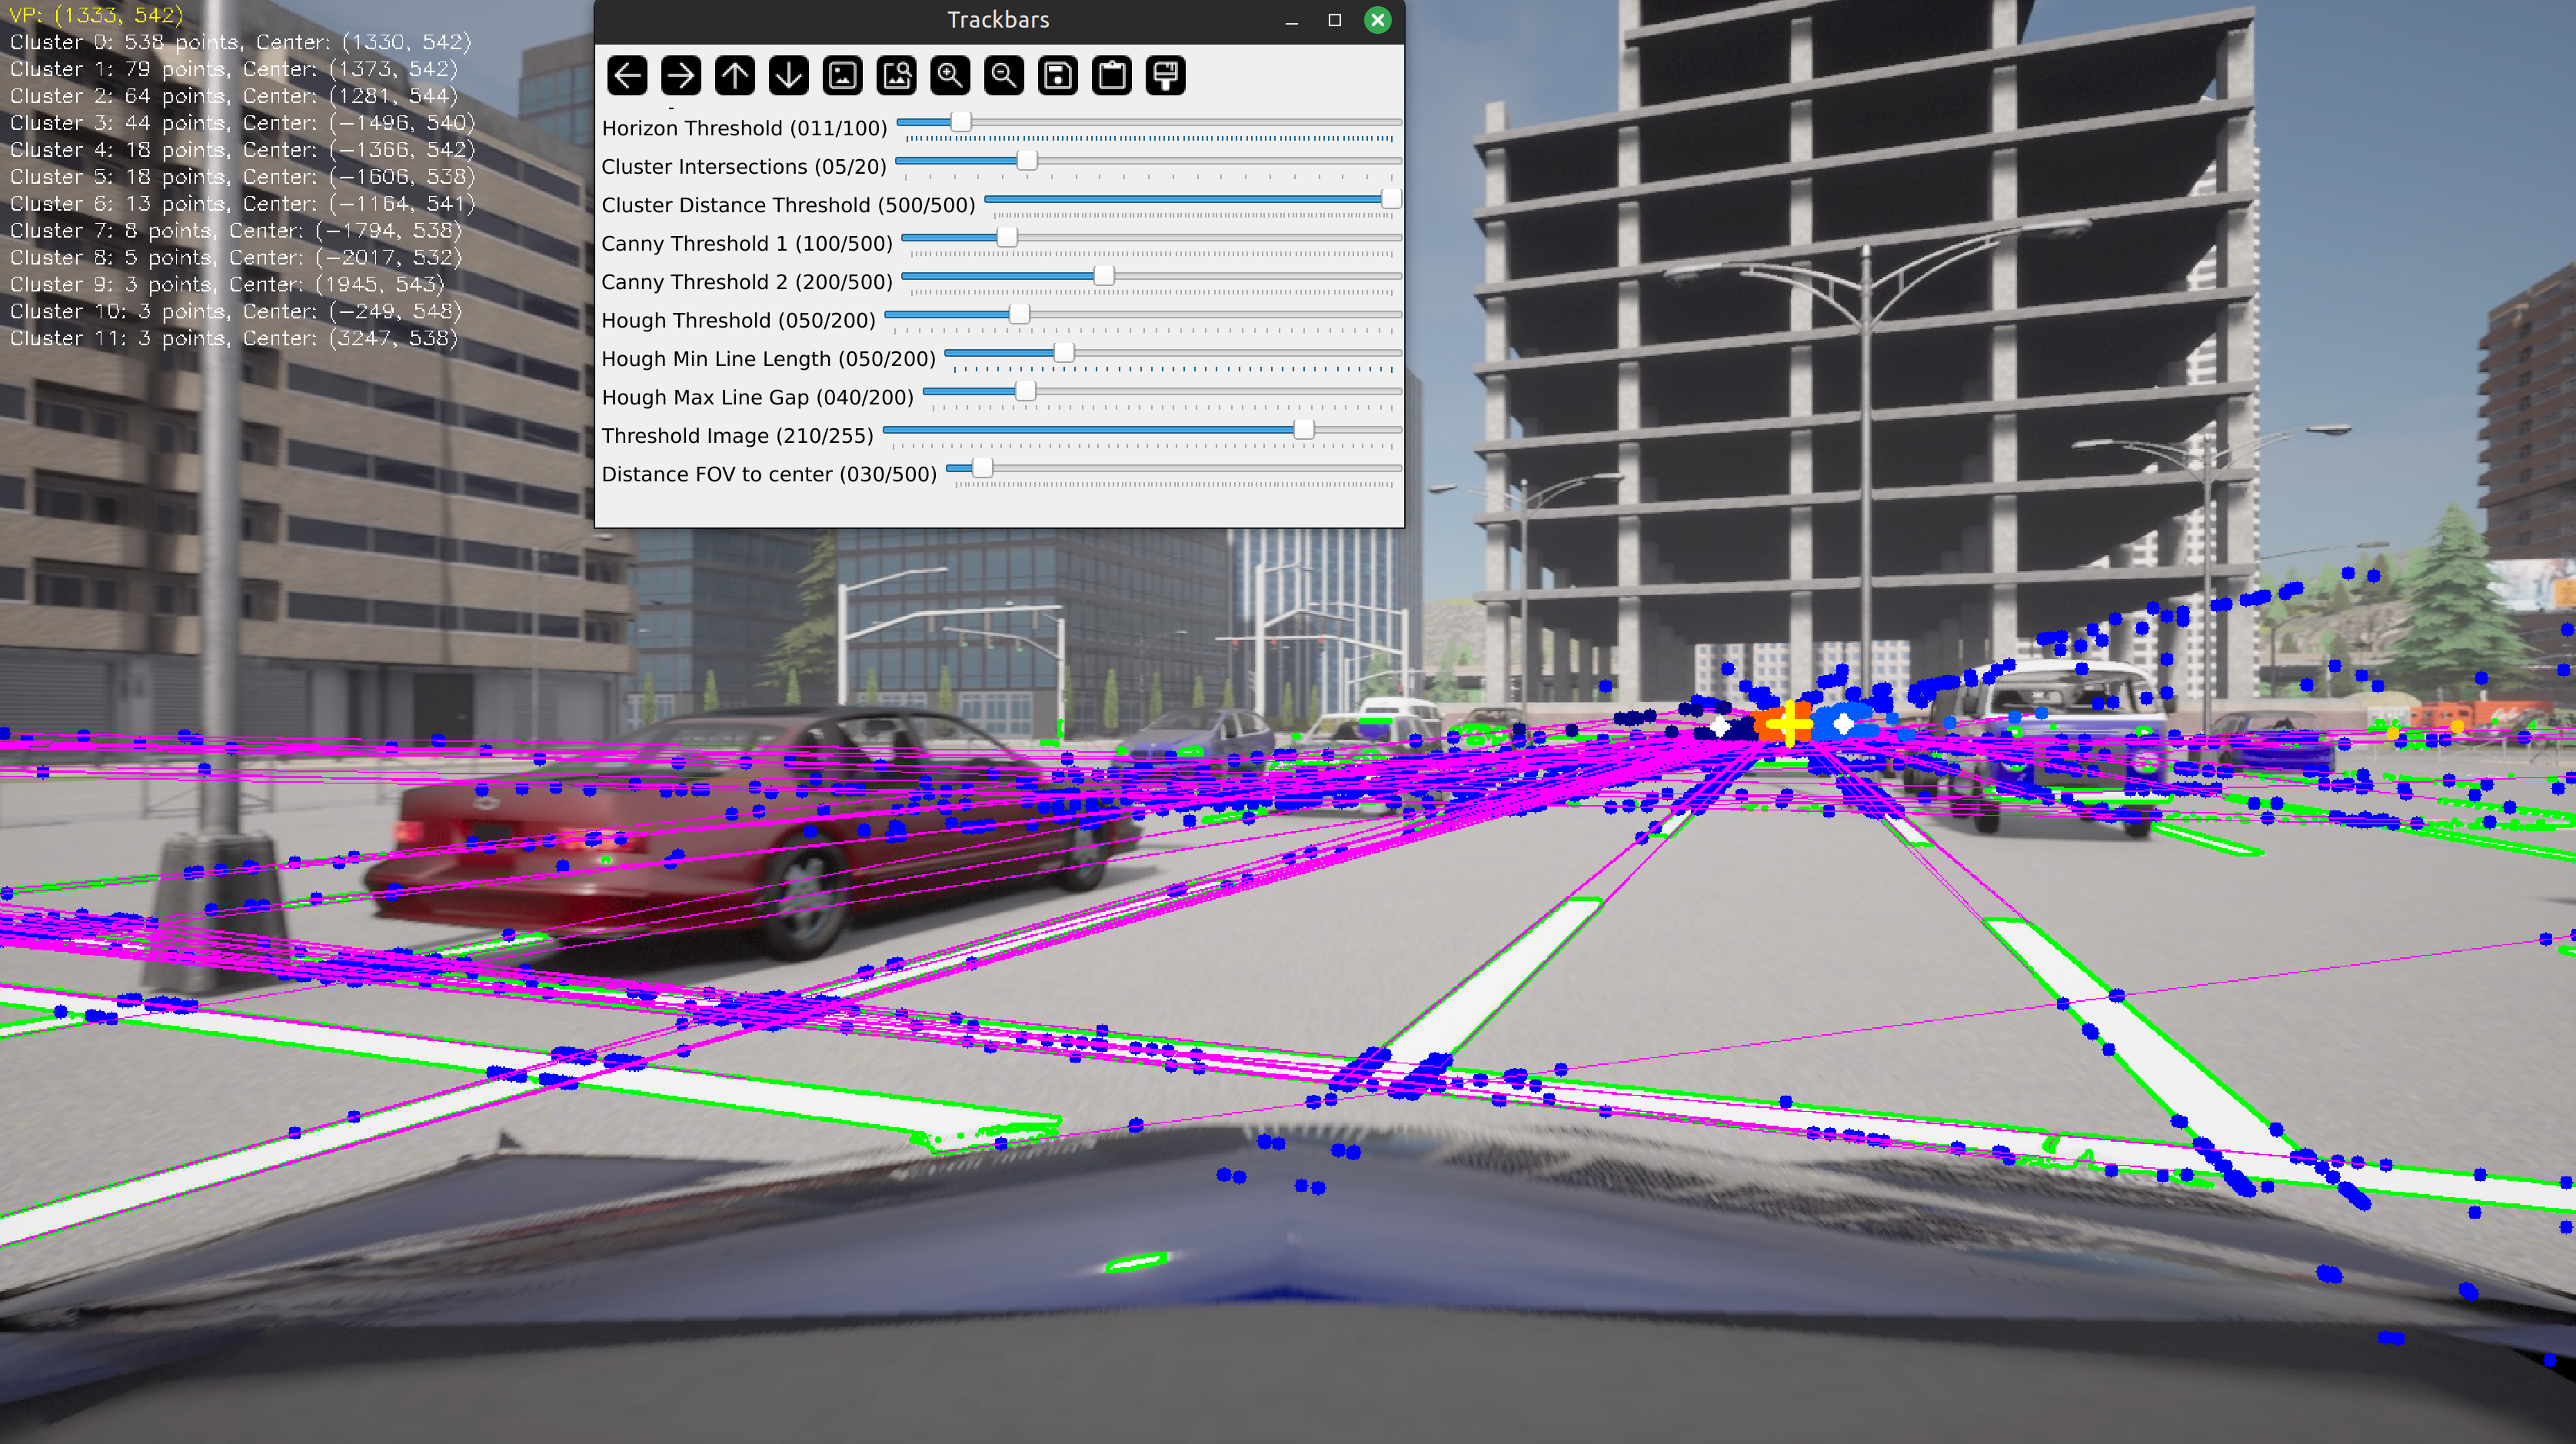
\includegraphics[width=\textwidth]{img/reticule/experimentationRgb}
	% 	\caption{Ejemplo de experimentación (RGB)}
	% 	\label{fig:experimentationRgb-teo}
	% \end{subfigure}
	
		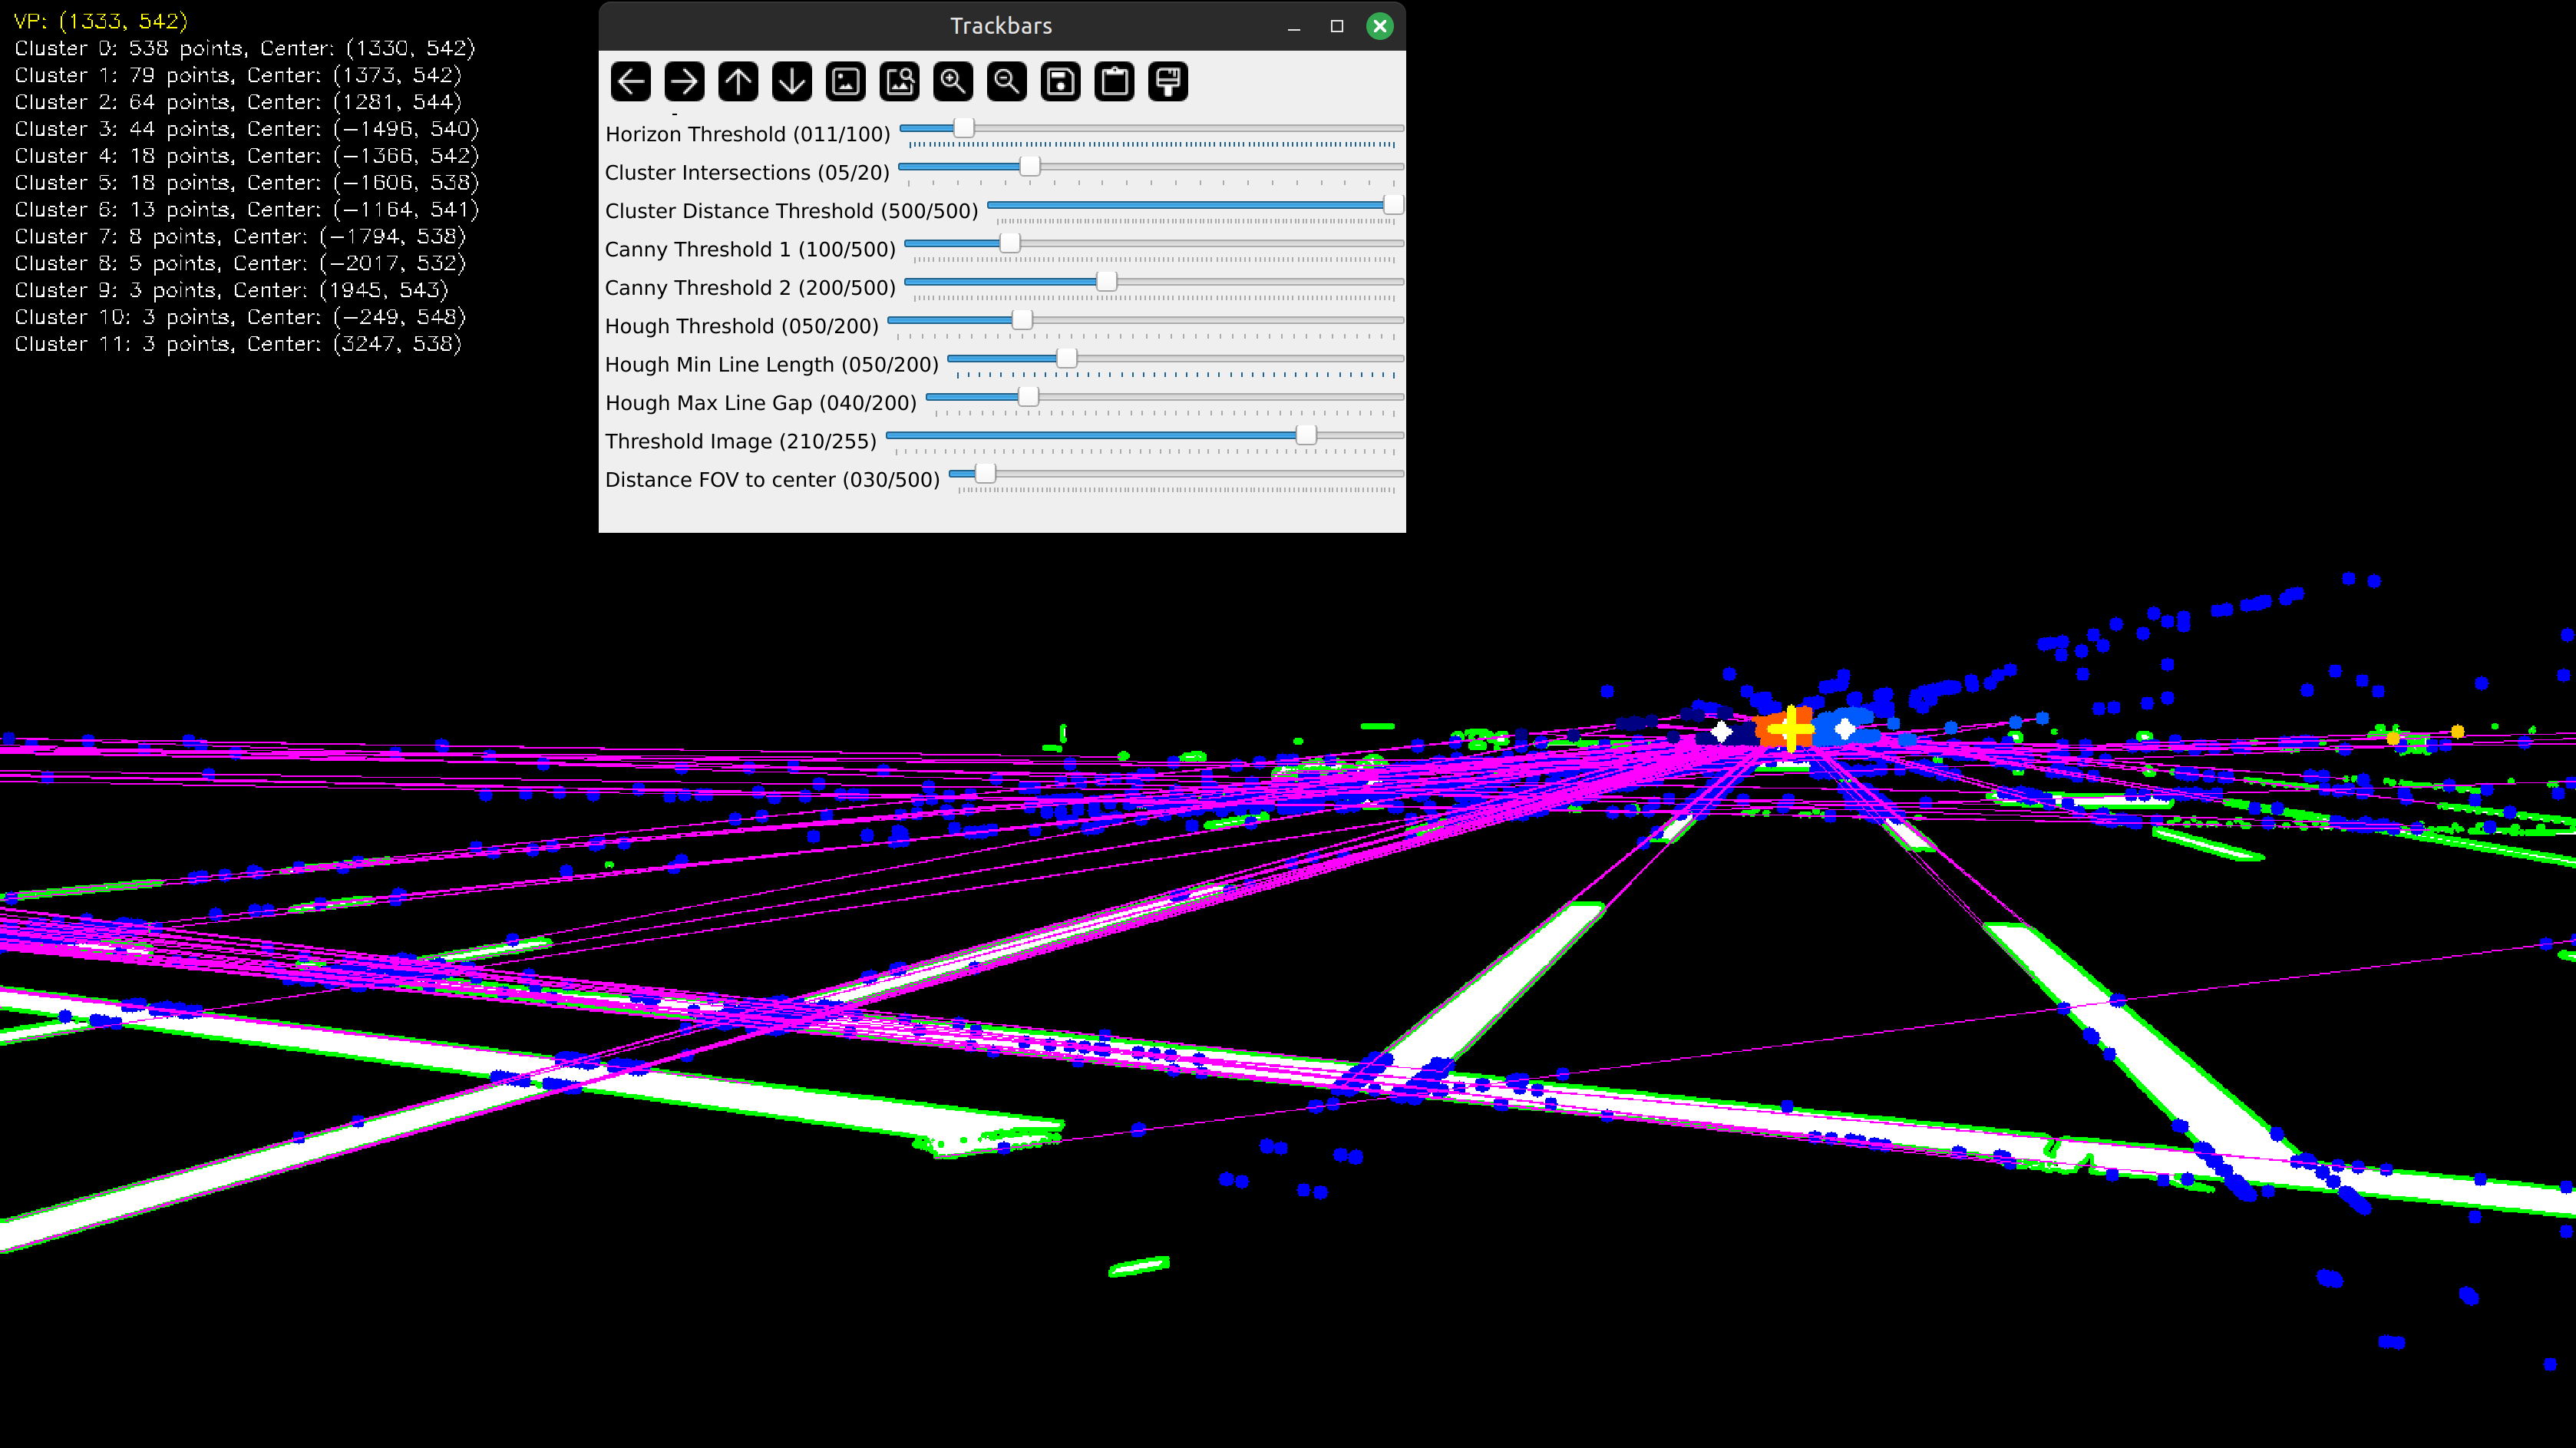
\includegraphics[width=0.8\textwidth]{img/reticule/experimentationBinary}
		\caption{Ejemplo de experimentación (Binaria)}
		\label{fig:experimentationBinary-teo}
	
\end{figure}


La interfaz incorpora una "Trackbar" para modificar parámetros en tiempo real y observar su efecto inmediato,
facilitando la búsqueda de configuraciones estables y robustas para distintas condiciones de escena.


% Capítulo 3: Metodología
\clearpage
\chapter{Metodología}\label{chap:metodologia}
\noindent
Este capítulo describe cómo se aplican en la práctica los conceptos del marco teórico 
para estimar la retícula de estacionamiento. Primero se detalla la configuración del 
entorno de simulación en CARLA (Sección \ref{sec:carla}). 
Luego se aborda el preprocesado: área de interés, umbralización, 
Canny y Hough (Sección \ref{sec:canny-hough}), seguido de la estimación de puntos de fuga 
y el filtrado de intersecciones y líneas relevantes. A partir de ello, 
se ejecuta el bucle RANSAC propuesto: muestreo de líneas por punto de fuga, cálculo de intersecciones 
(candidato a cajón), estimación de la homografía hacia un cuadrado 1×1, proyección de una retícula n×n 
y evaluación del error respecto a las líneas reales; al finalizar, se selecciona la homografía con menor 
error como representación de la retícula (Sección \ref{sec:metodo-reticula}). Por último, se presenta la 
construcción de la representación de la posición relativa y los criterios de validación experimental.

\section{Entorno de simulación}\label{sec:carla}

De acuerdo con lo expuesto en la sección \ref{sec:plataformas},
empleamos CARLA como entorno de simulación para nuestros experimentos.
El escenario de estacionamiento incluye un vehículo con el objetivo de estacionarse y un área con cajones marcados.
La posición inicial del vehículo se varía de forma controlada entre ejecuciones.
La cámara frontal se monta en la zona del retrovisor a altura conocida,
y se recopilan secuencias de imágenes para alimentar el pipeline de detección de líneas,
estimación de puntos de fuga y ajuste de retícula por RANSAC.
La Figura~\ref{fig:simulation-design} muestra un ejemplo del diseño del entorno.

\begin{figure}[!ht]
    \centering
    \begin{subfigure}{0.4\textwidth}
        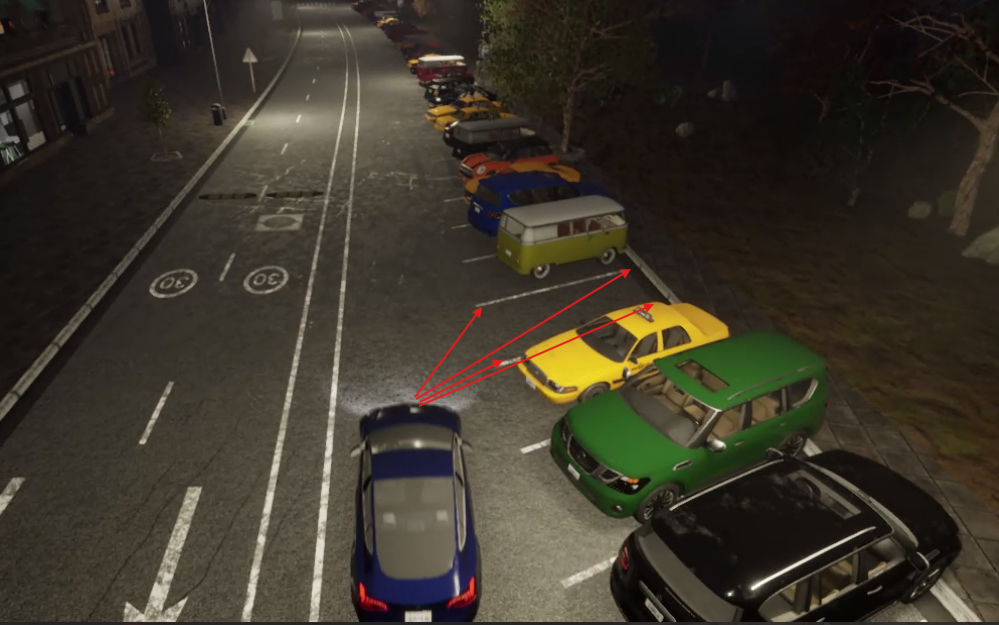
\includegraphics[width=\textwidth]{img/distances}\label {fig:distances}
    \end{subfigure}
    \begin{subfigure}{0.4\textwidth}
        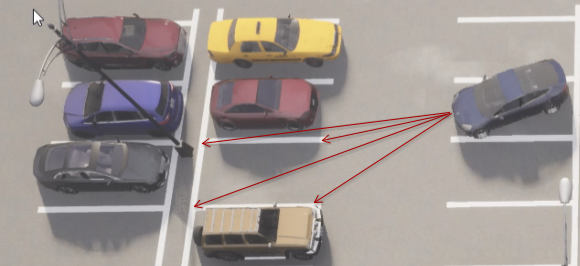
\includegraphics[width=\textwidth]{img/distances2}\label {fig:distances2}
    \end{subfigure}

    \caption{Diseño del entorno de simulación en CARLA.}
    \label{fig:simulation-design}
\end{figure}


La Figura~\ref{fig:camera-view} ilustra ejemplos de la vista de la cámara frontal desde la ubicación definida.

\begin{figure}[!ht]
    \centering
    \begin{subfigure}{0.4\textwidth}
        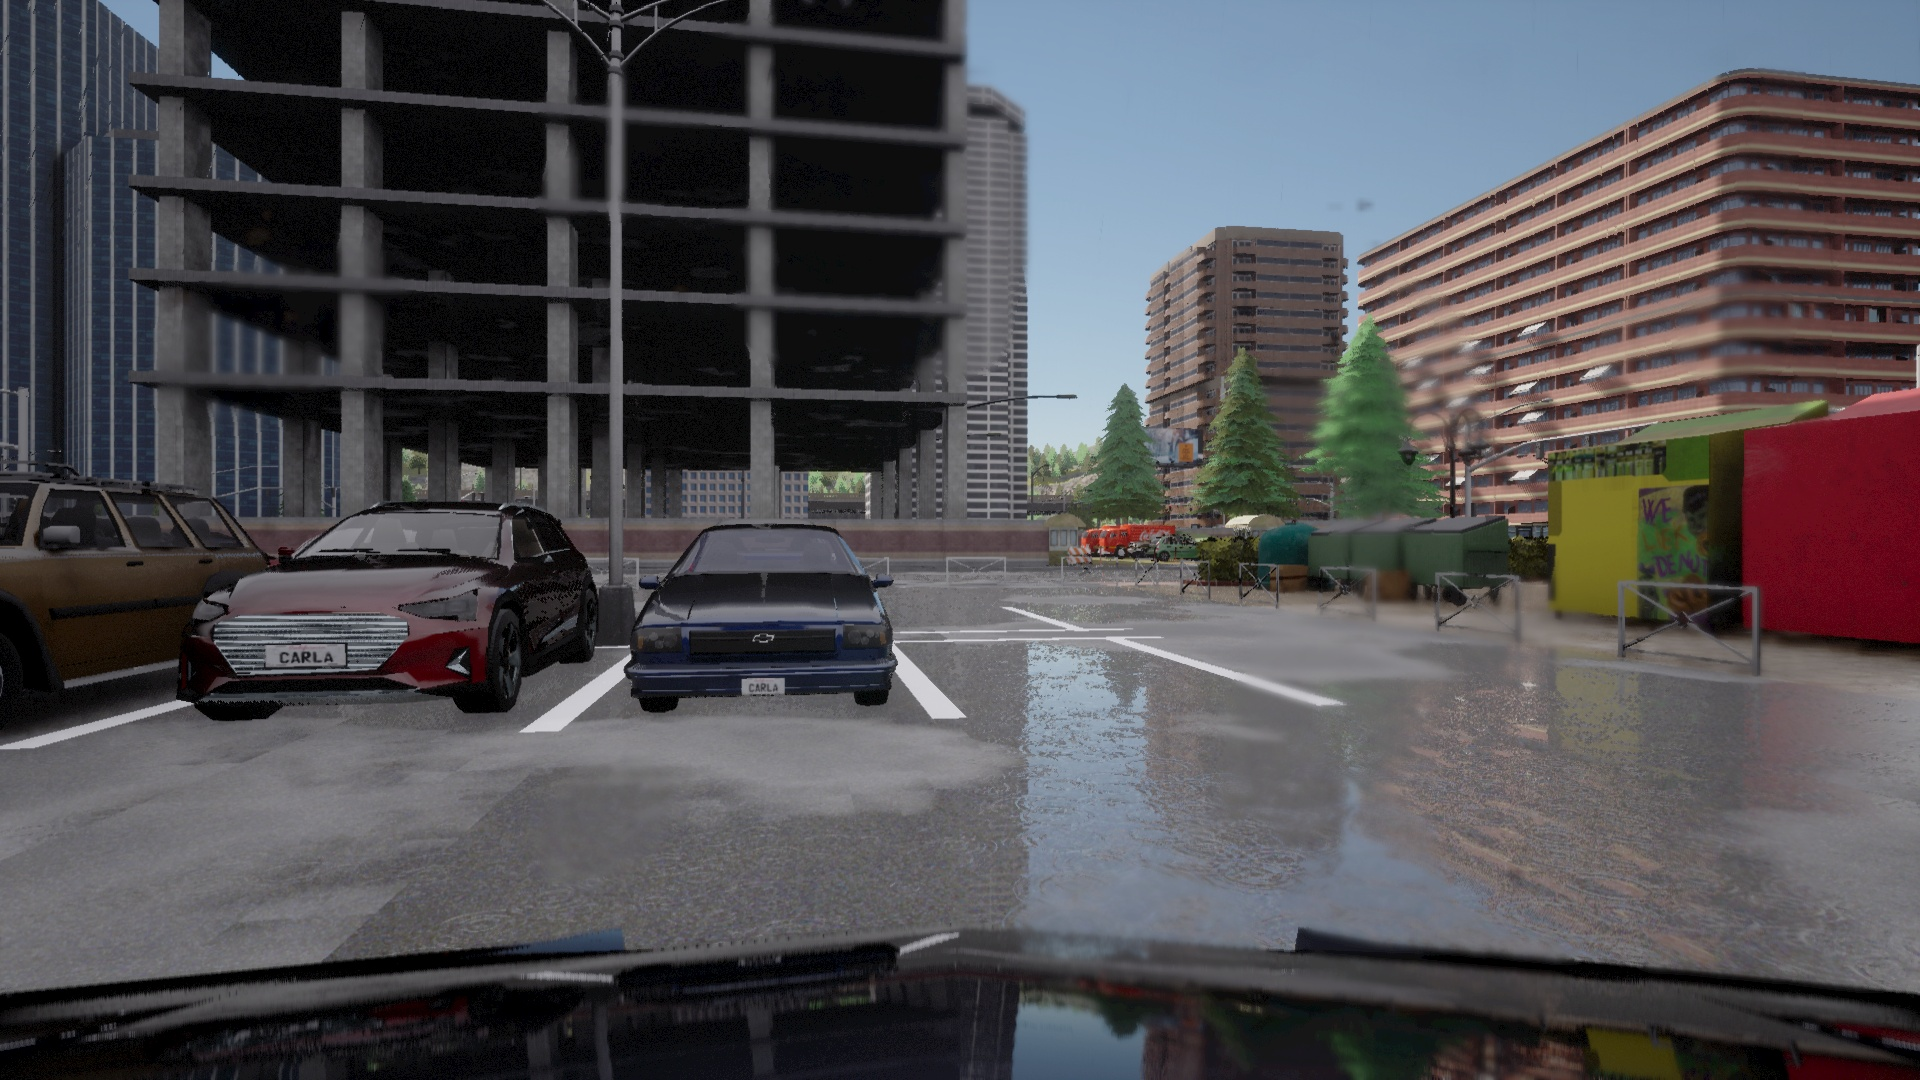
\includegraphics[width=\textwidth]{img/mirrow_camara_ex}\label {fig:camara}
    \end{subfigure}
    \begin{subfigure}{0.4\textwidth}
        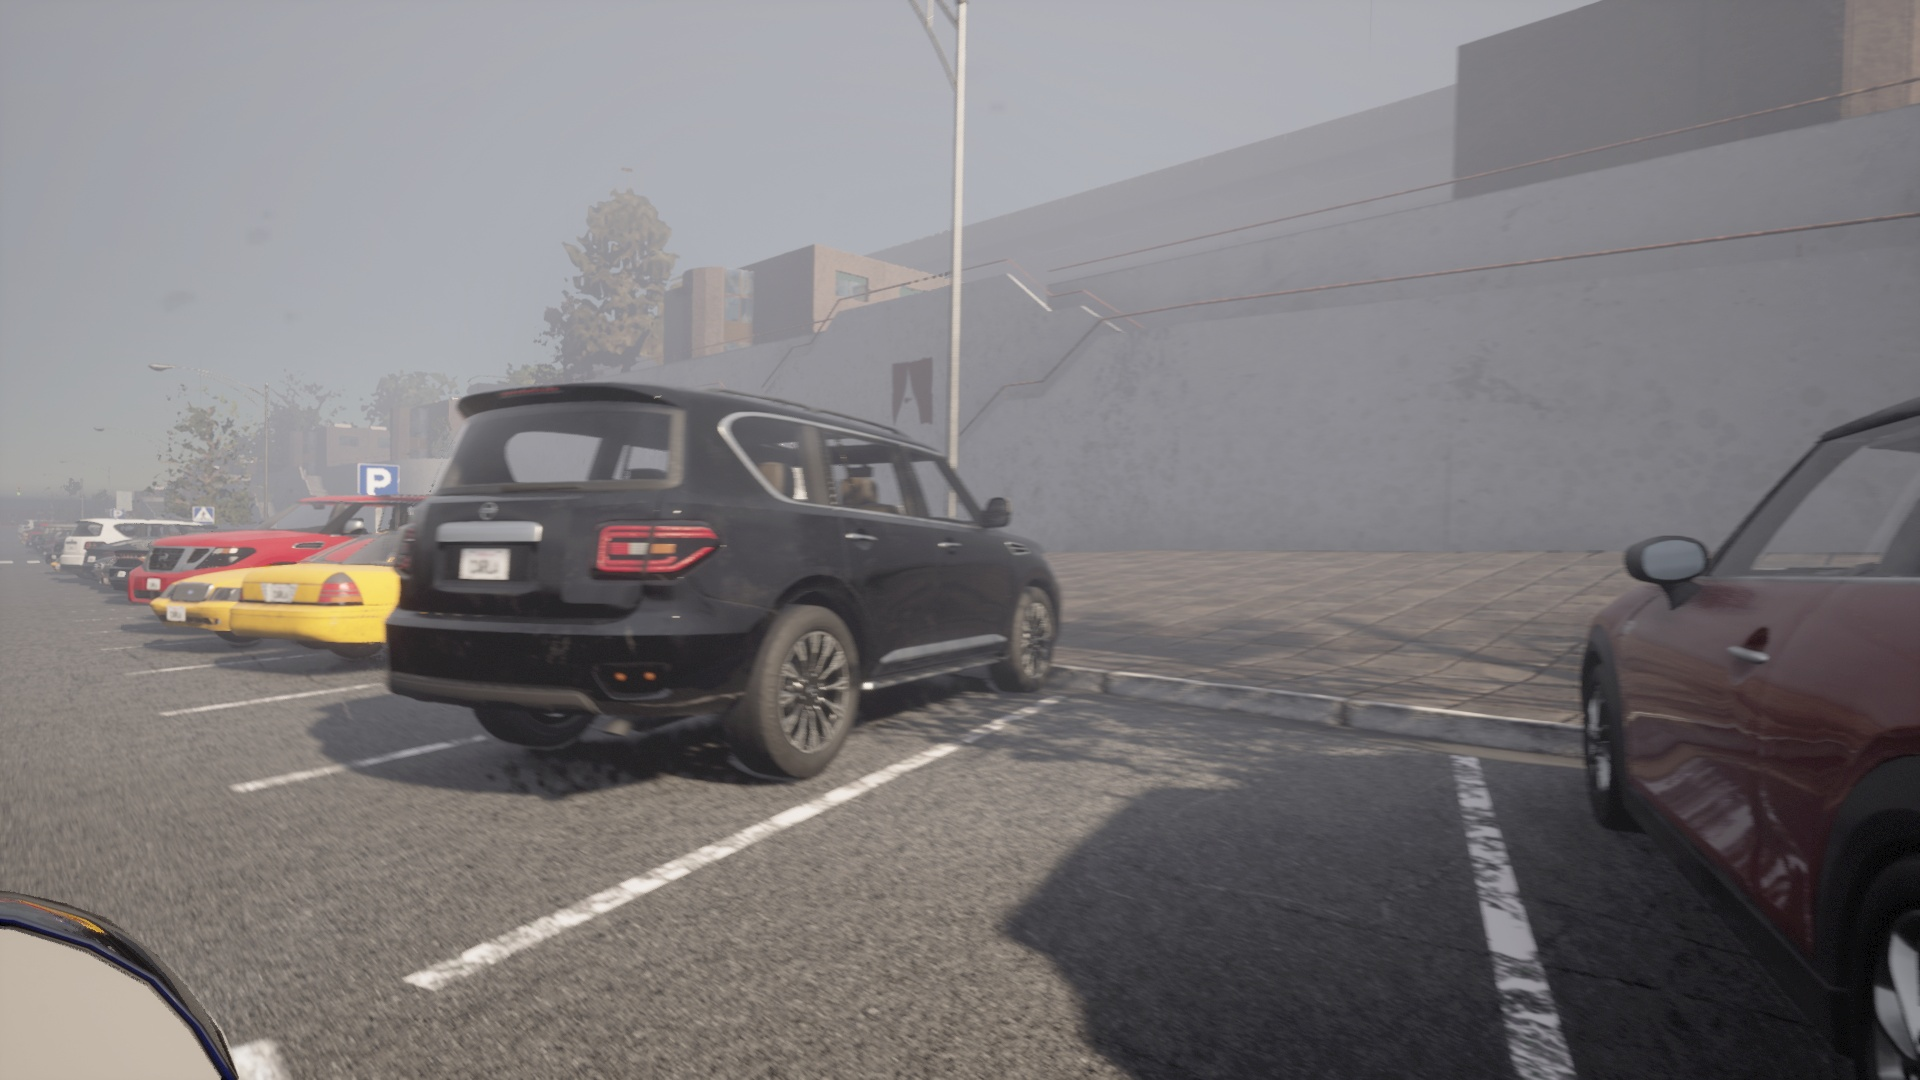
\includegraphics[width=\textwidth]{img/mirrow_camara_ex2}\label {fig:camara2}
    \end{subfigure}
    \caption{Vista de la cámara en el entorno de simulación.}
    \label{fig:camera-view}
\end{figure}






\section{Detección de la retícula de estacionamiento}\label{sec:metodo-reticula}
\noindent
En esta sección desarrollamos el procedimiento práctico para detectar la
retícula de estacionamiento a partir de una imagen de la cámara frontal.
Nos apoyamos en los fundamentos del Marco teórico: Canny y Hough (Sección~\ref{sec:canny-hough}),
la representación de rectas y su intersección en coordenadas homogéneas
(Sección~\ref{sec:rectas-svd}), y los puntos de fuga (Sección~\ref{sec:vanishing-points}).
\noindent
Partimos de una imagen RGB capturada por la cámara frontal. Trabajamos sobre una región de interés (ROI)
definida por debajo del horizonte excluyendo la franja superior para reducir ruido.
Como resultado del procesamiento, obtenemos conjuntos de líneas agrupados según su punto de fuga y un conjunto de esquinas candidatas a vértices de cajón. Dada la naturaleza de la escena, pueden presentarse dificultades como baja textura o contraste, oclusiones y marcas del pavimento degradadas; para mitigarlas, empleamos umbrales ajustables y reintentos por cuadro.

\noindent
Por la proyección perspectiva, las líneas paralelas del mundo se intersectan en la imagen en un punto de fuga
(véase Sección~\ref{sec:vanishing-points} y Fig.~\ref{fig:distorion-teo}).
En nuestro contexto, las marcas de los cajones son aproximadamente paralelas y generan
una retícula de paralelogramos; esto habilita usar la detección de líneas para identificar puntos de fuga
y estimar la posición de la retícula.


\begin{figure}[!ht]
    \centering
    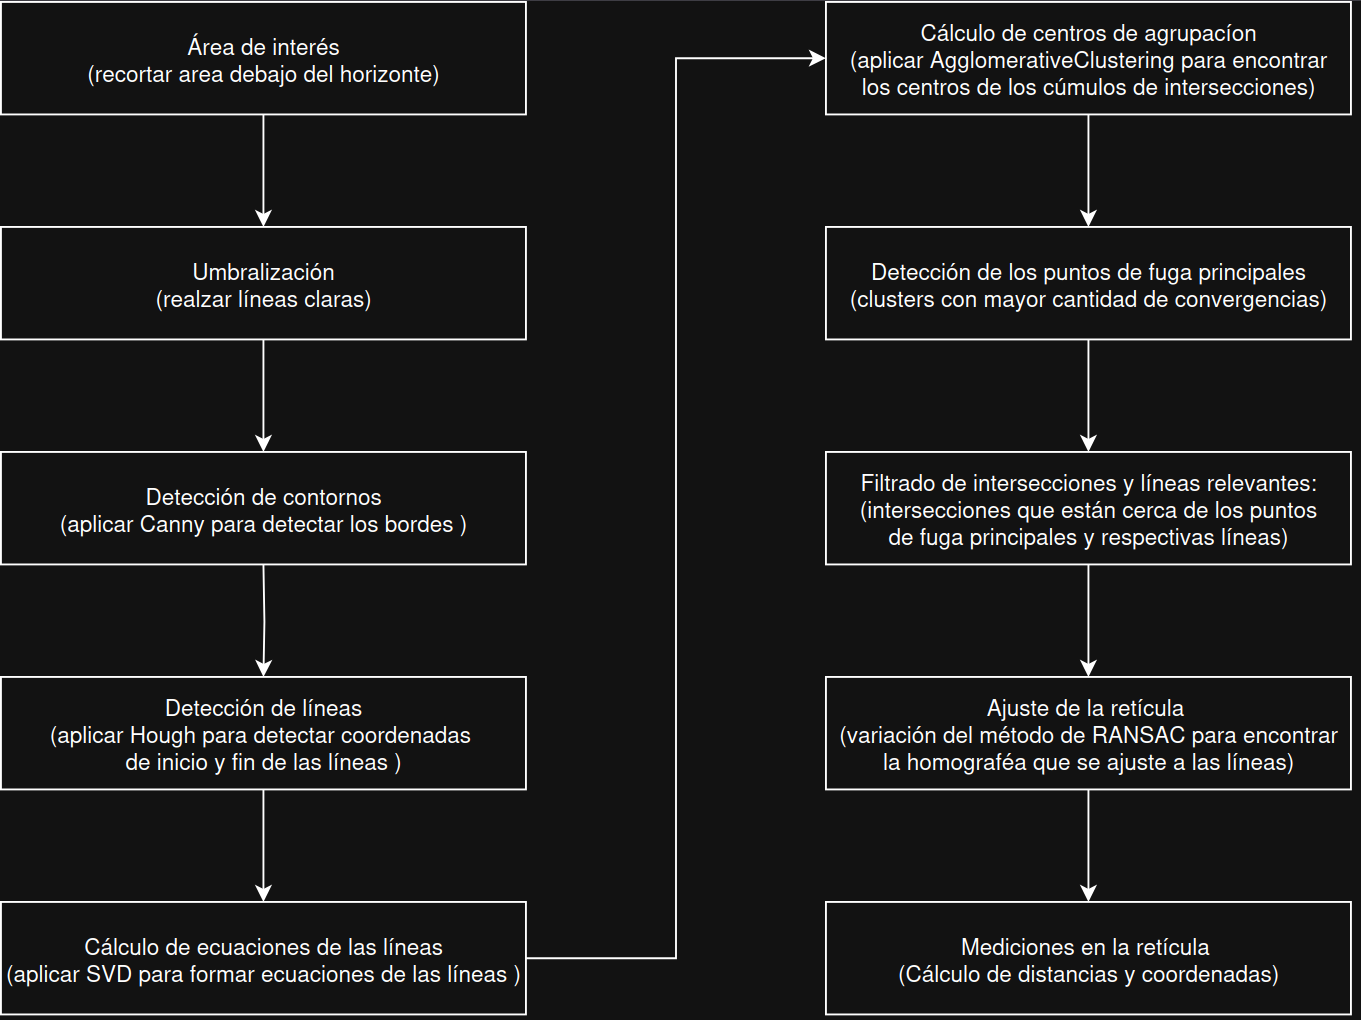
\includegraphics[width=0.8\textwidth]{img/3-metodo/piperline-reticule.png}
    \caption{Diagrama general del pipeline para la detección de la retícula de estacionamiento.}
    \label{fig:reticula-pipeline}
\end{figure}

\noindent
A continuación, desarrollamos cada etapa del diagrama de la Figura~\ref{fig:reticula-pipeline},
centrándonos en el procesamiento de imagen y la extracción de información geométrica relevante con técnicas clásicas de visión computacional.


\subsubsection{Área de interés:}
\noindent
Teniendo en cuenta que la cámara del vehículo se encuentra ubicada en la parte delantera a una altura conocida y en un ángulo paralelo al suelo, el área de interés de la imagen donde se encuentran las líneas de los cajones de estacionamiento quedará siempre por debajo del horizonte de la imagen.
Por lo tanto, se puede eliminar la parte superior de la imagen para
reducir el ruido y mejorar la detección de las líneas, como se muestra en la figura \ref{fig:roi}. \\
\begin{figure}[!ht]
    \centering
    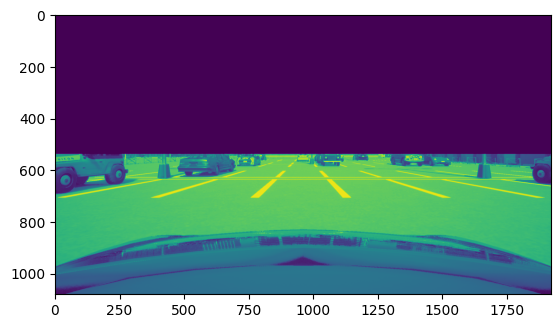
\includegraphics[width=0.9\textwidth]{img/reticule/horizont}
    \caption{Área de interés de la imagen}
    \label{fig:roi}
\end{figure}

\subsubsection{Umbralización:}
\noindent
Al área de interés de la imagen se le aplica una umbralización para realzar las líneas blancas de los cajones de estacionamiento
y eliminar otros elementos no relevantes que puedan interferir en la detección.
En la figura \ref{fig:threshold} se muestra un ejemplo de la imagen umbralizada.
\begin{figure}[!ht]
    \centering
    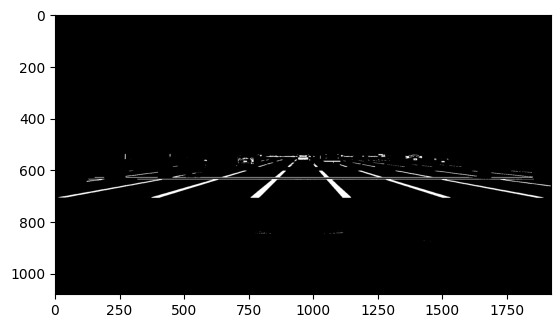
\includegraphics[width=0.9\textwidth]{img/reticule/thresholded}
    \caption{Imagen umbralizada}
    \label{fig:threshold}
\end{figure}

\subsubsection{Detección de contornos (Canny):}
\noindent
Se utiliza el algoritmo de Canny \cite{canny1986edge} (véase Sección~\ref{sec:canny-hough}) para detectar los bordes de las líneas en la imagen umbralizada.
En la figura \ref{fig:edges} se muestra un ejemplo de la imagen con los bordes detectados.
\begin{figure}[!ht]
    \centering
    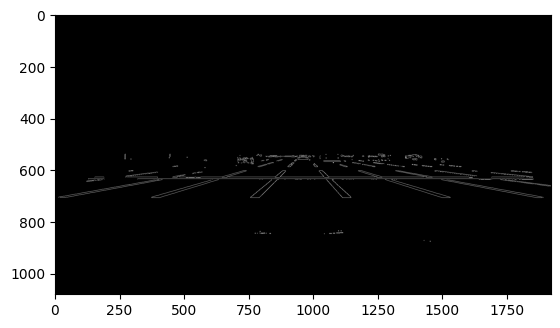
\includegraphics[width=0.9  \textwidth]{img/reticule/canny}
    \caption{Detección de bordes mediante el algoritmo de Canny}
    \label{fig:edges}
\end{figure}

\subsubsection{Detección de líneas (Hough):}
\noindent
Se aplica la transformada de Hough \cite{ballard1981hough} (Sección~\ref{sec:canny-hough}) para detectar las coordenadas de inicio y fin de las líneas en la imagen.
En las figuras \ref{fig:hough} y \ref{fig:lines} se muestran las líneas detectadas sin fondo y sobre la imagen original, respectivamente.
\begin{figure}[!ht]
    \begin{subfigure}{0.5\textwidth}
        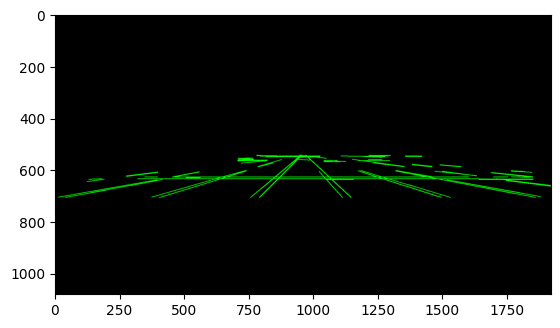
\includegraphics[width=\textwidth]{img/reticule/hough2}
        \caption{Líneas detectadas con la transformada de Hough}
        \label{fig:hough}
    \end{subfigure}
    \begin{subfigure}{0.5\textwidth}
        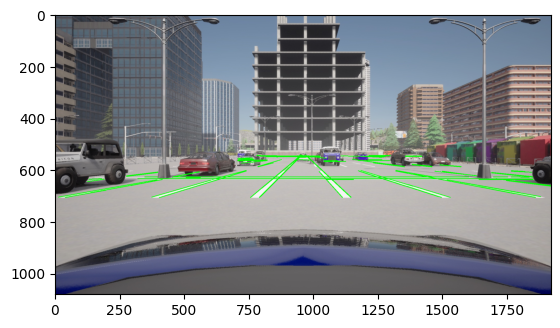
\includegraphics[width=\textwidth]{img/reticule/hough}
        \caption{Líneas detectadas en la imagen original}
        \label{fig:lines}
    \end{subfigure}
\end{figure}

\subsubsection{Representación de las ecuaciones de las líneas:}
\noindent
Una vez obtenidas las coordenadas de inicio y fin de cada línea paralela, se puede utilizar la ecuación general de la recta (véase Sección~\ref{sec:rectas-svd}):
\begin{equation}
    Ax + By + C = 0
\end{equation}
Esta ecuación permite determinar la orientación de cada línea.
Dado que las coordenadas iniciales y finales de cada línea corresponden a los valores de $x$ y $y$, respectivamente,
estas se pueden emplear para formular un sistema de ecuaciones que describa los parámetros de la recta $[A, B, C]$.
Dicho sistema puede representarse de manera matricial como sigue:
\begin{equation}
    \begin{aligned}
        \left[\begin{array}{ccc}
                      x_1 & y_1 & 1 \\
                      x_2 & y_2 & 1
                  \end{array}\right]
        \begin{bmatrix}
            A \\
            B \\
            C
        \end{bmatrix}
        =
        \begin{bmatrix}
            0 \\
            0
        \end{bmatrix}
    \end{aligned}
\end{equation}
\noindent
Esta representación permite calcular de forma precisa los coeficientes de la ecuación de la recta para cada línea detectada,
lo cual es fundamental para analizar su orientación y posición dentro de la retícula de estacionamiento.

\subsubsection{Cálculo de ecuaciones de las líneas (SVD):}
\noindent
Para calcular los coeficientes $[A, B, C]$ de las ecuaciones de las líneas detectadas, se utiliza el concepto de espacio nulo (\emph{null space}) y SVD (Sección~\ref{sec:rectas-svd}).
Este enfoque se basa en el hecho de que cualquier vector en el espacio nulo de una matriz $\mathbf{M}$ satisface la ecuación
\begin{equation}
    \mathbf{Mv} = 0
\end{equation}

\noindent
Cada línea se representa mediante dos puntos $(x_1, y_1)$ y $(x_2, y_2)$. A partir de estas coordenadas homogéneas,
se construye una matriz $\mathbf{M}$ de la forma:
\[
    \mathbf{M} = \begin{bmatrix}
        x_1 & y_1 & 1 \\
        x_2 & y_2 & 1
    \end{bmatrix}
\]
Esta matriz define el sistema de ecuaciones que describe la recta que pasa por los puntos dados.
El espacio nulo de $\mathbf{M}$ corresponde al conjunto de vectores $[A,B,C]$ que satisfacen
\[
    \mathbf{M} \cdot \begin{bmatrix}
        A \\ B \\ C
    \end{bmatrix} = \mathbf{0}.
\]
Se utiliza la Descomposición en Valores Singulares (SVD) \cite{golub2013matrix} para calcular este espacio nulo, ya que es una herramienta robusta y numéricamente estable.
La SVD descompone la matriz \(M\) en tres matrices \(U\), \(S\) y \(V\), donde el espacio nulo de \(M\) se puede obtener a partir de la última columna de la matriz \(V\), que corresponde al vector singular más pequeño (el más cercano a cero).
El vector resultante del espacio nulo se normaliza para que tenga una magnitud manejable.
Esto asegura que los coeficientes \(A\), \(B\) y \(C\) sean comparables entre distintas líneas.

\subsubsection{Cálculo de intersecciones (Clustering):}
\noindent
Una vez que se tienen las ecuaciones de todas las líneas paralelas en el plano de la cámara, se pueden calcular las intersecciones de estas líneas realizando un producto cruz entre las ecuaciones homogéneas [\(A\),\(B\),\(C\)] de todos los pares de líneas.
\noindent
El resultado de este producto cruz es la coordenada homogénea de un punto en el espacio que corresponde a la intersección de las líneas.
Si este punto es finito (cuando la tercera componente no es cero), se puede deshomogeneizar para obtener las coordenadas cartesianas en el plano de la cámara.
En cambio, si el punto es infinito (cuando la tercera componente es muy cercana a cero), significa que las líneas son paralelas y se intersectan en el infinito.

%https://scikit-learn.org/stable/modules/clustering.html#hierarchical-clustering
\noindent
Analizando los puntos de intersección obtenidos que se encuentran en el plano de la cámara, se pueden agrupar para determinar dónde está
concentrada la mayor cantidad de intersecciones.
Este punto de concentración de intersecciones debe corresponder al punto de fuga principal de la retícula de estacionamiento.
En la figura \ref{fig:intersections} se muestra un ejemplo de las intersecciones detectadas en la imagen original,
donde cada color representa un cluster diferente y el símbolo \texttt{+} blanco indica el centro de cada cluster.
\\

\begin{figure}[!ht]
    \centering
    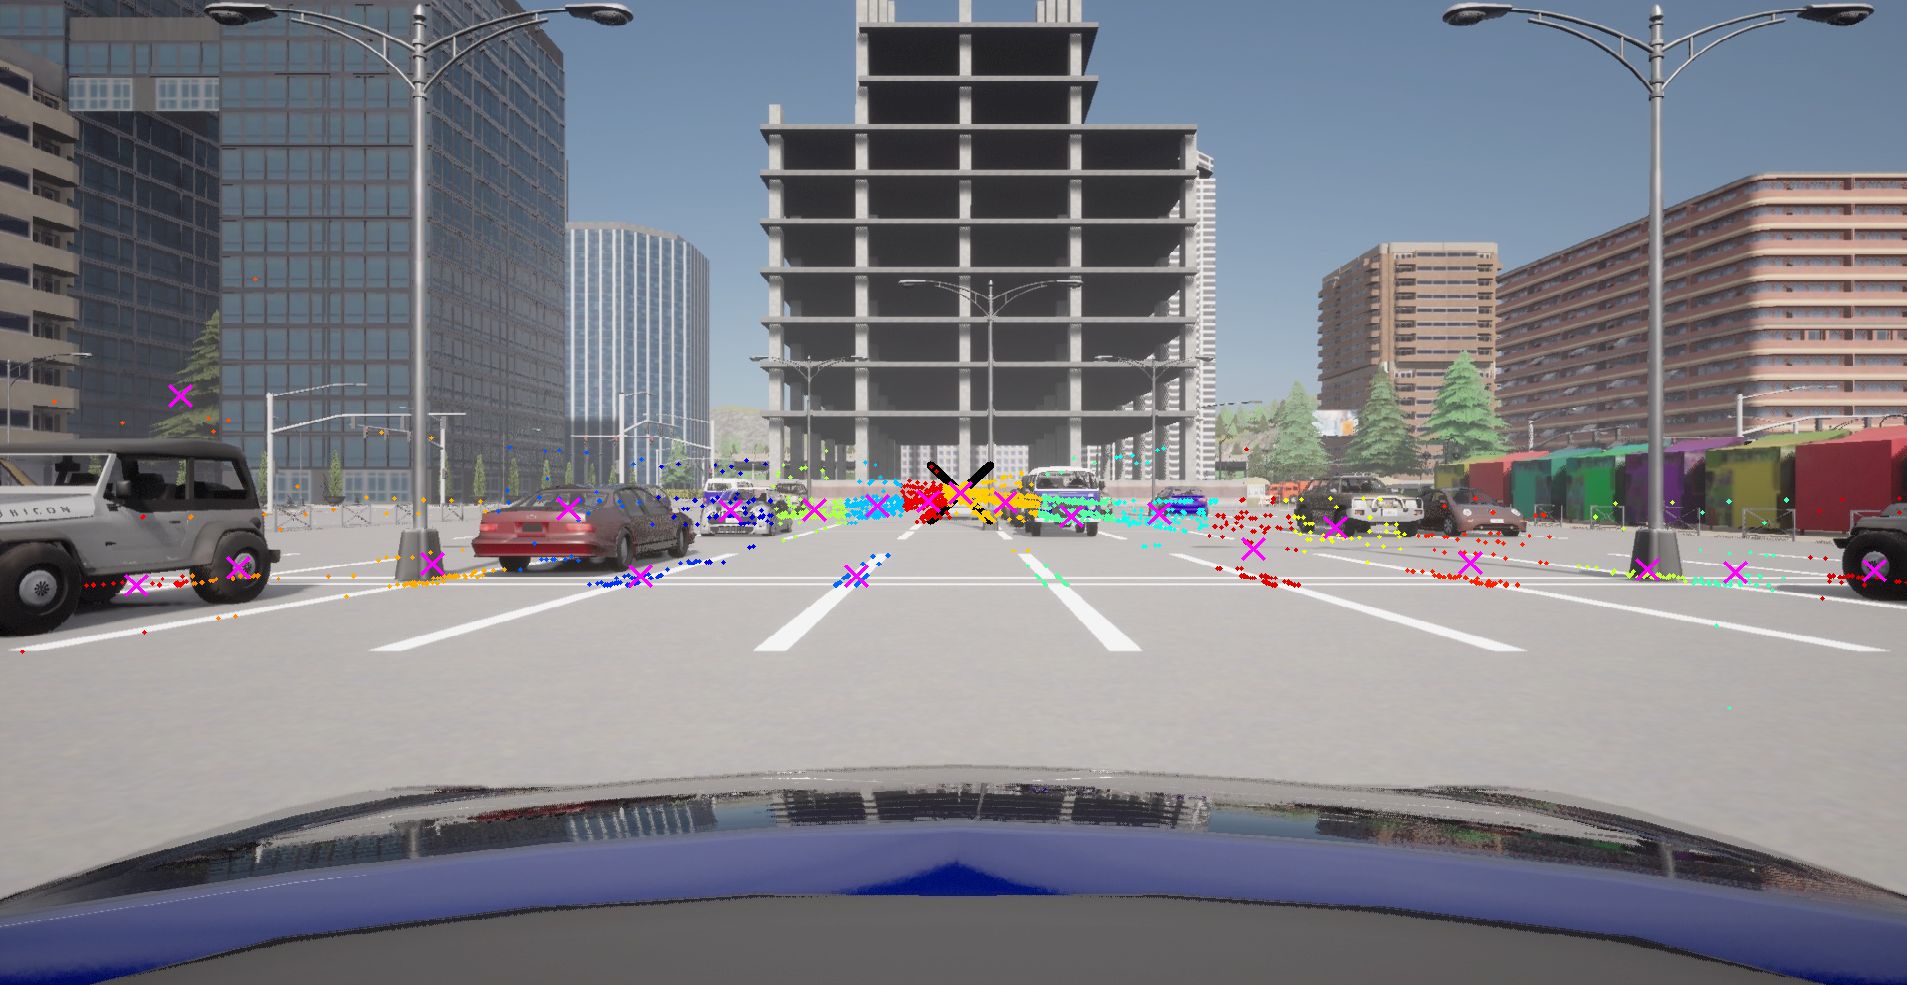
\includegraphics[width=0.9\textwidth]{img/reticule/svd-km}
    \caption{Agrupacion de intersecciones de las líneas detectadas}
    \label{fig:intersections}
\end{figure}
\noindent
Como se discute en la Sección~\ref{sec:intersections-clustering}, para estimar la ubicación de este punto de fuga principal no es necesario tener en cuenta todas las intersecciones detectadas, sino solo aquellas que se encuentran en una zona cercana al horizonte de la imagen (Sección~\ref{sec:vanishing-points}).
Para determinar las intersecciones relevantes cercanas al horizonte, se puede definir un umbral de cercanía en la imagen que se puede ajustar experimentalmente.
Por ejemplo, en la siguiente imagen se muestran las intersecciones detectadas en la imagen original con puntos azules
y las intersecciones relevantes con un umbral de 10 píxeles con puntos amarillos.
En la figura \ref{fig:relevantInter} se muestra el resultado de la selección de las intersecciones relevantes. \\
\begin{figure}[!ht]
    \centering
    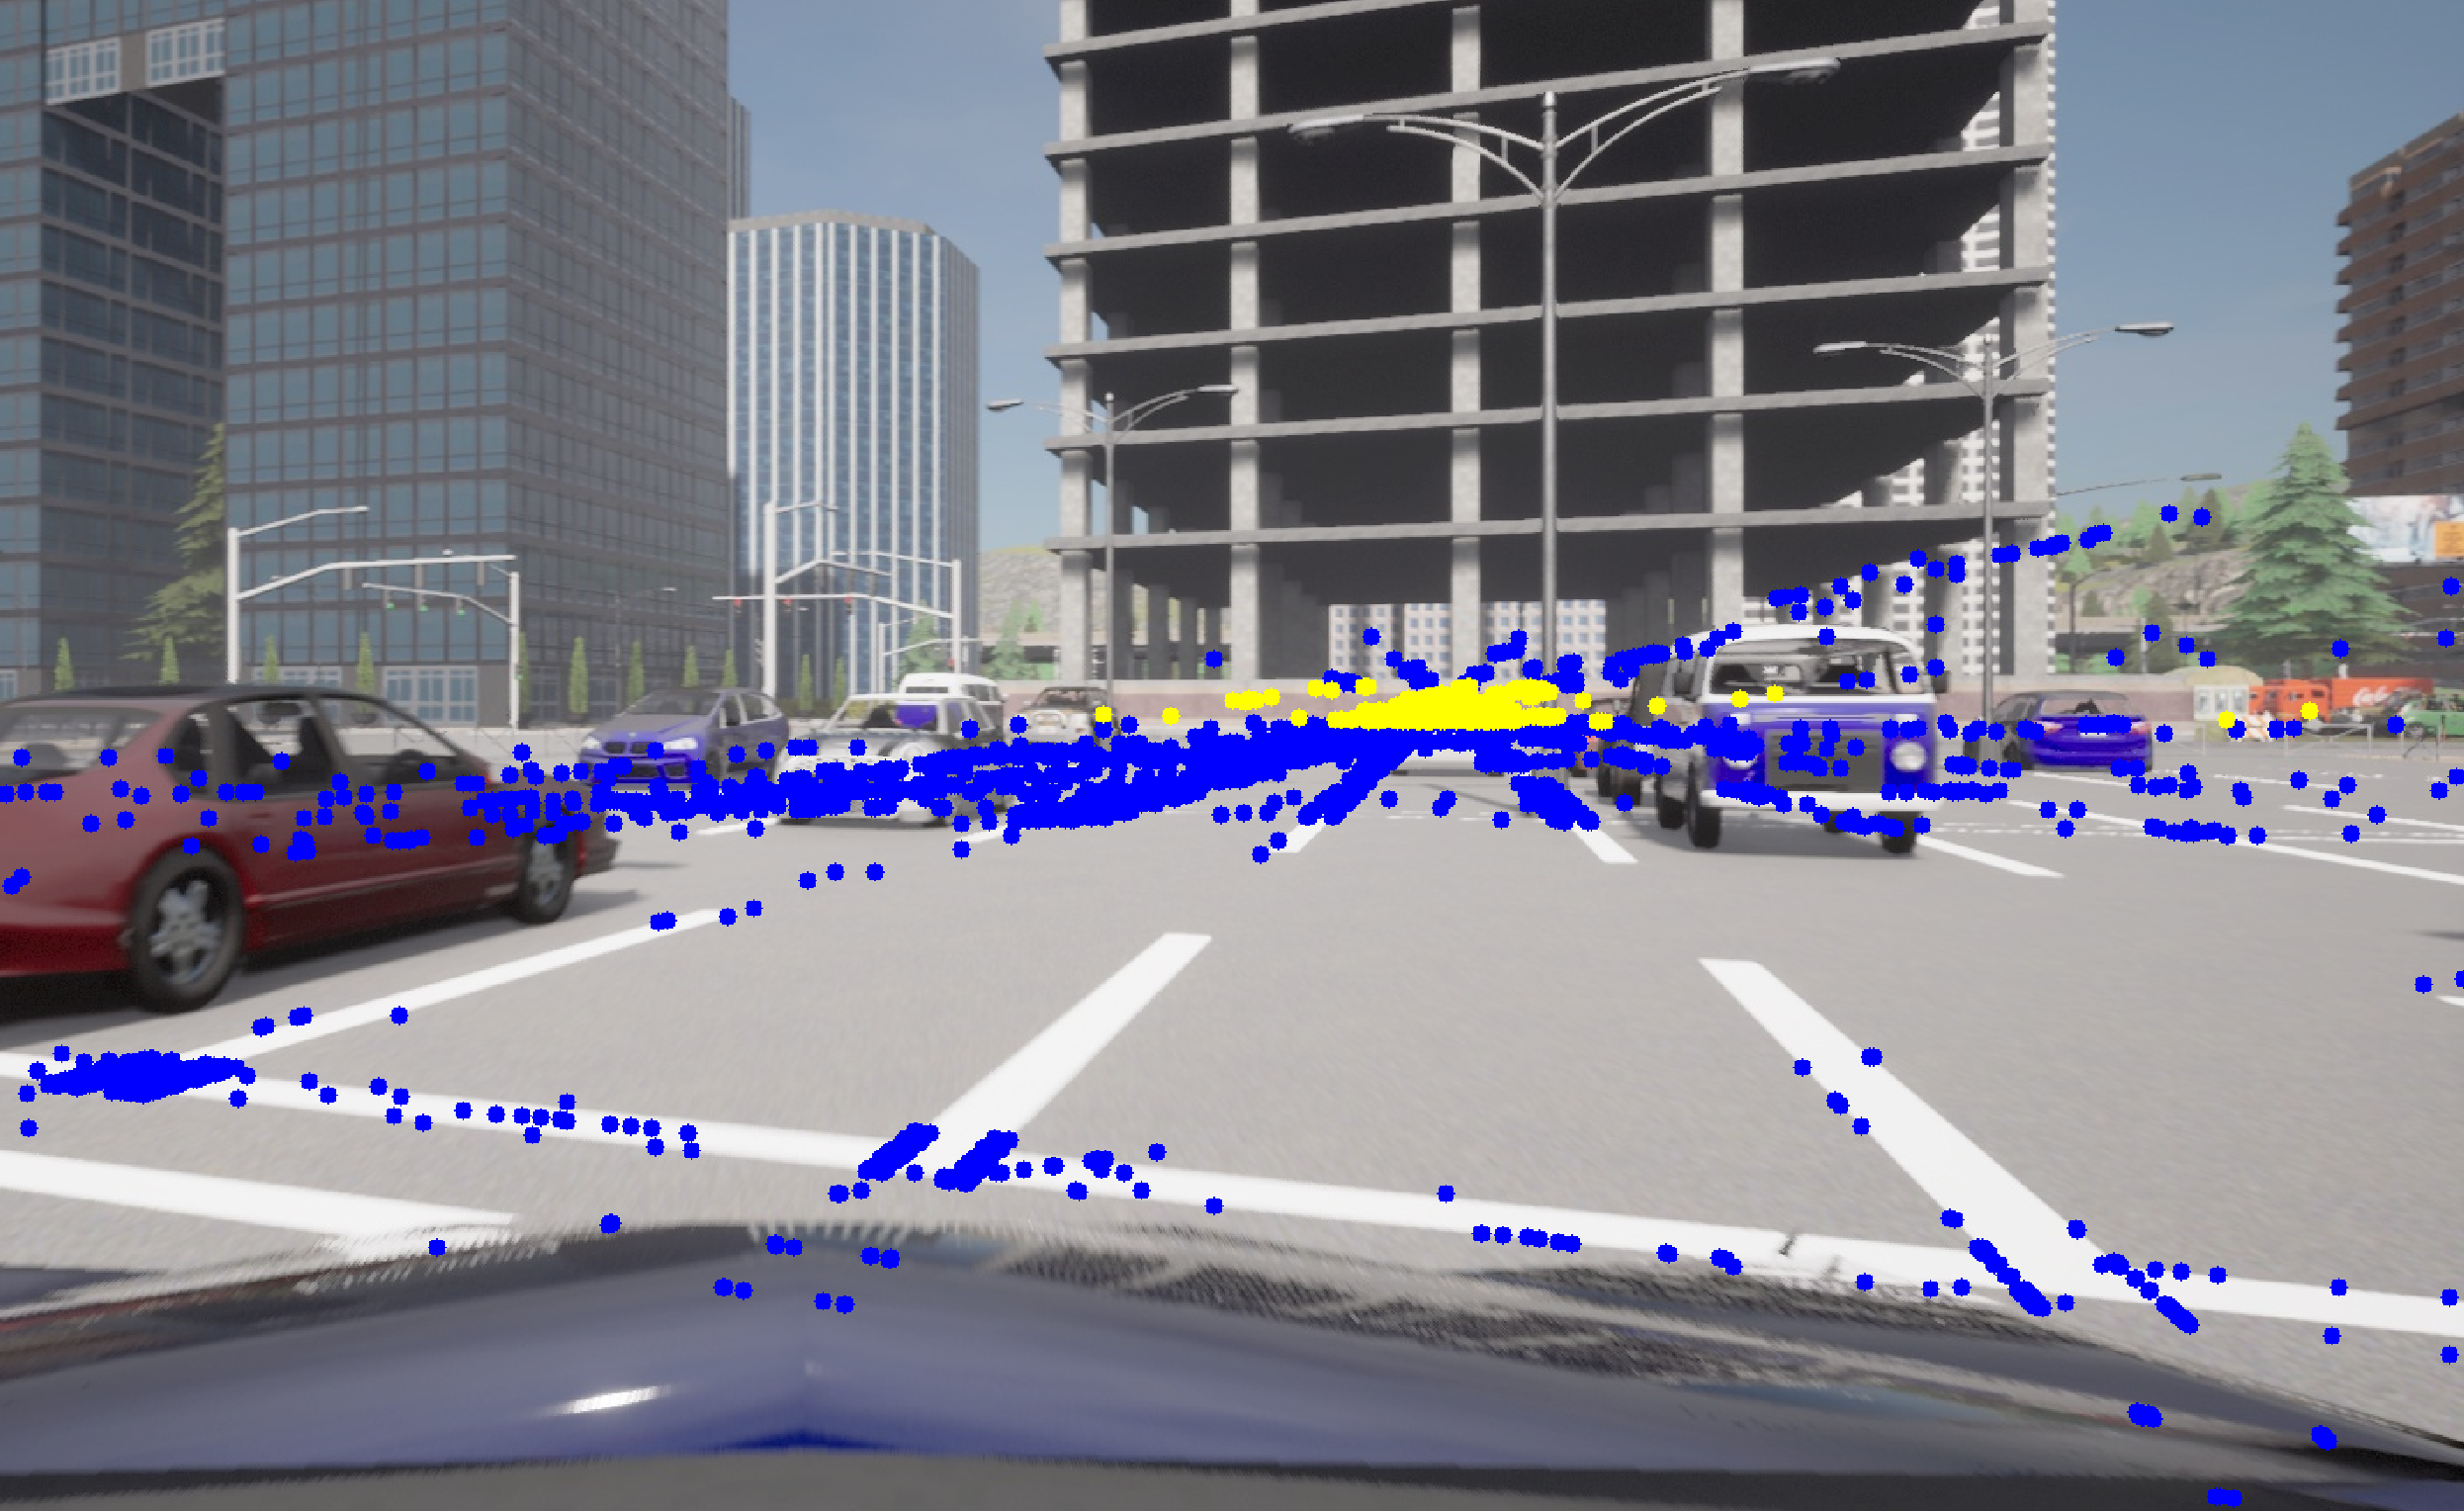
\includegraphics[width=0.9\textwidth]{img/reticule/relevantInter}
    \caption{Intersecciones detectadas en la imagen original}
    \label{fig:relevantInter}
\end{figure}

\noindent
Para agrupar las intersecciones relevantes empleamos \texttt{AgglomerativeClustering} de \texttt{scikit-learn}
(véase Sección~\ref{sec:sklearn-agglomerative}). En nuestra configuración práctica,
dejamos que el algoritmo determine el número de clusters fijando \texttt{distance\_threshold} (distancia máxima entre puntos del mismo
cluster), cuyo valor se ajusta experimentalmente al escenario. A continuación se ilustra el resultado sobre las mismas
intersecciones relevantes del ejemplo anterior: se forman 3 clusters (colores distintos) y se marca con \texttt{+} blanco el centroide de cada uno
(Fig.~\ref{fig:clusters}).
\begin{figure}[!ht]
    \centering
    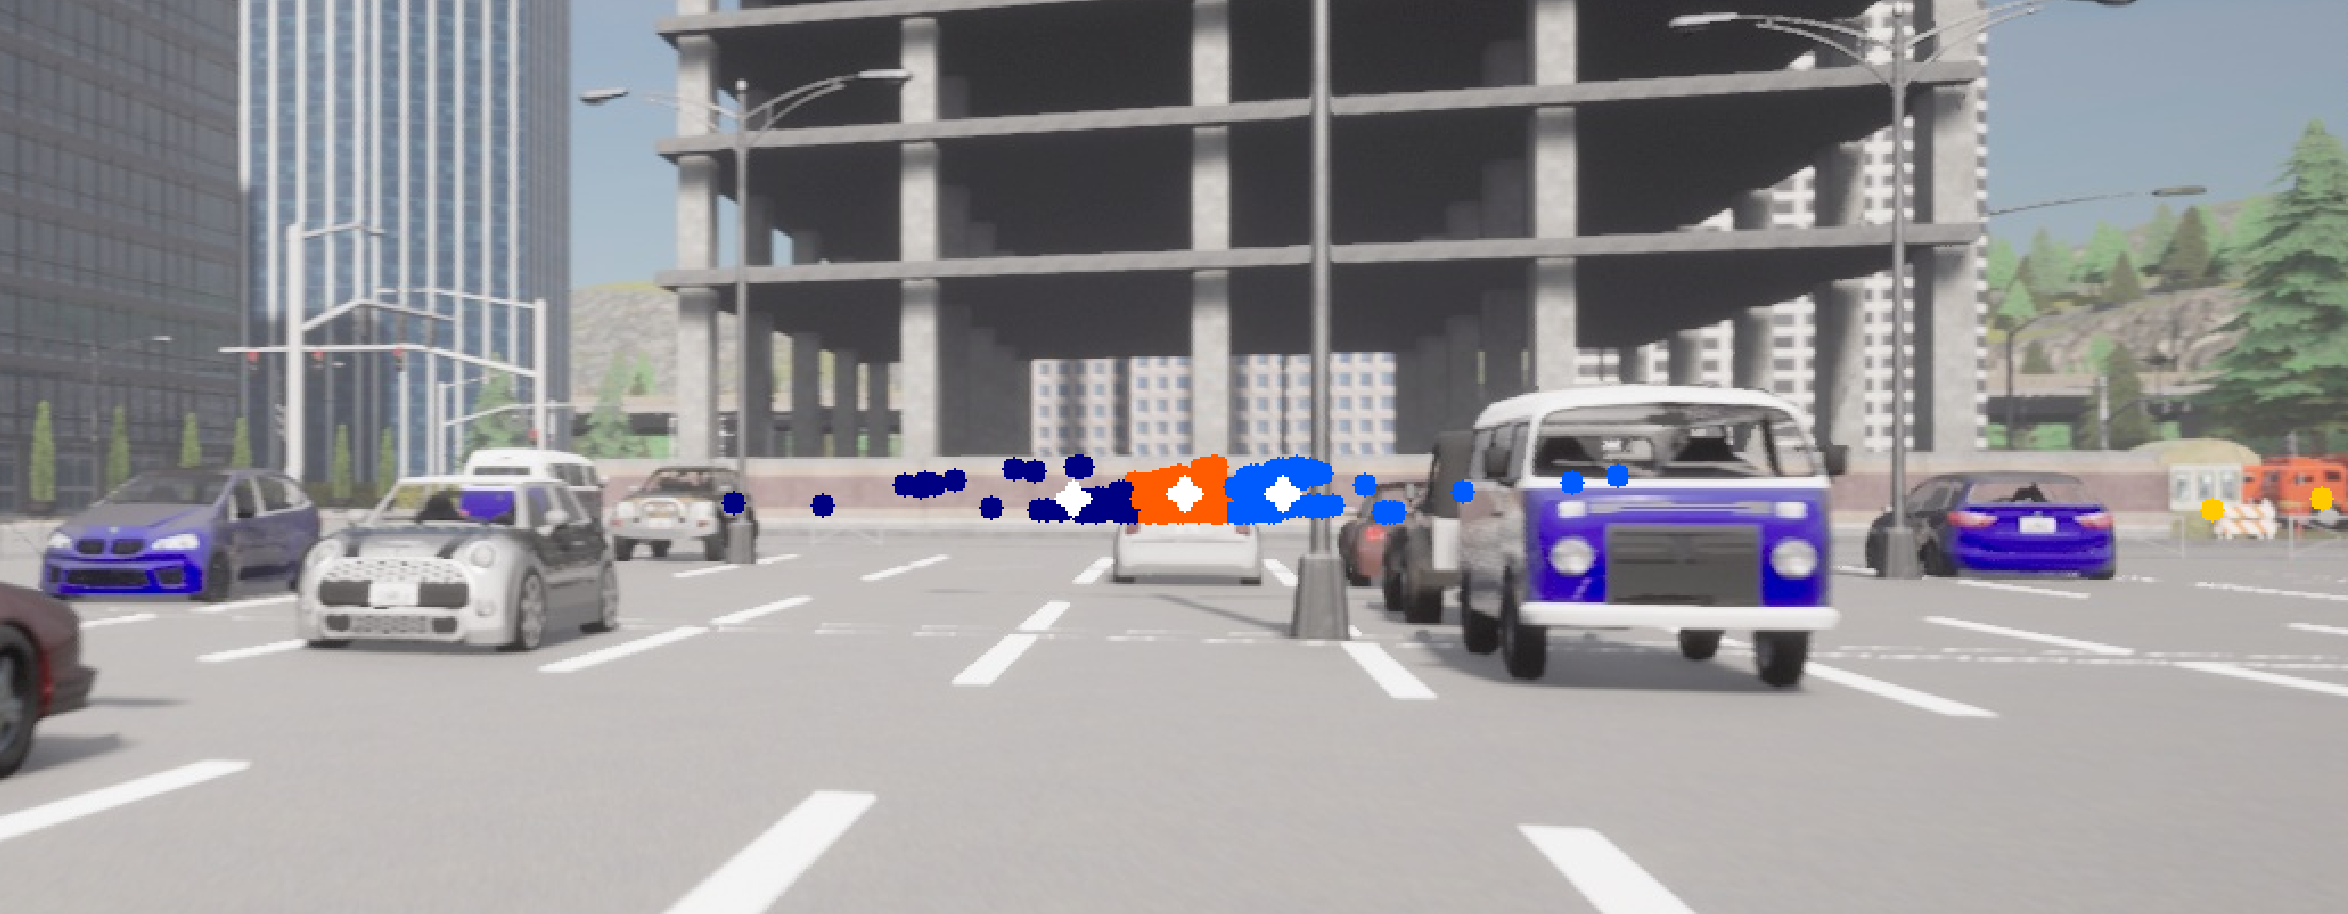
\includegraphics[width=0.9\textwidth]{img/reticule/AgglomerativeClustering}
    \caption{Intersecciones agrupadas en clusters}
    \label{fig:clusters}
\end{figure}



\subsubsection{Selección del punto de fuga principal:}
\noindent
Para estimar la posición del punto de fuga principal, se puede seleccionar el cluster con mayor cantidad de intersecciones y
utilizar las líneas que generaron estos puntos para calcular la intersección de estas líneas.
La intersección de $n$ líneas (bajo un criterio de mínimos cuadrados) está dada por
el eigenvector asociado al eigenvalor más pequeño de la matriz $M$, donde:
\[
    M = \sum_{i=1}^{n} w_i l_i l_i^T
\]
Aquí, $w_i$ es un peso asociado a la línea $l_i$ y $l_i$ es la representación homogénea de la línea $i$ \cite{kanatani1998statistical}.
De esta forma, podemos conocer la posición del punto de fuga principal en el plano de la cámara.
En la figura \ref{fig:vanishingPoint} se muestra el resultado de esta estimación utilizando las líneas del cluster más grande, donde se
representa el punto de fuga principal con un símbolo \texttt{+} amarillo.
\begin{figure}[!ht]
    \centering
    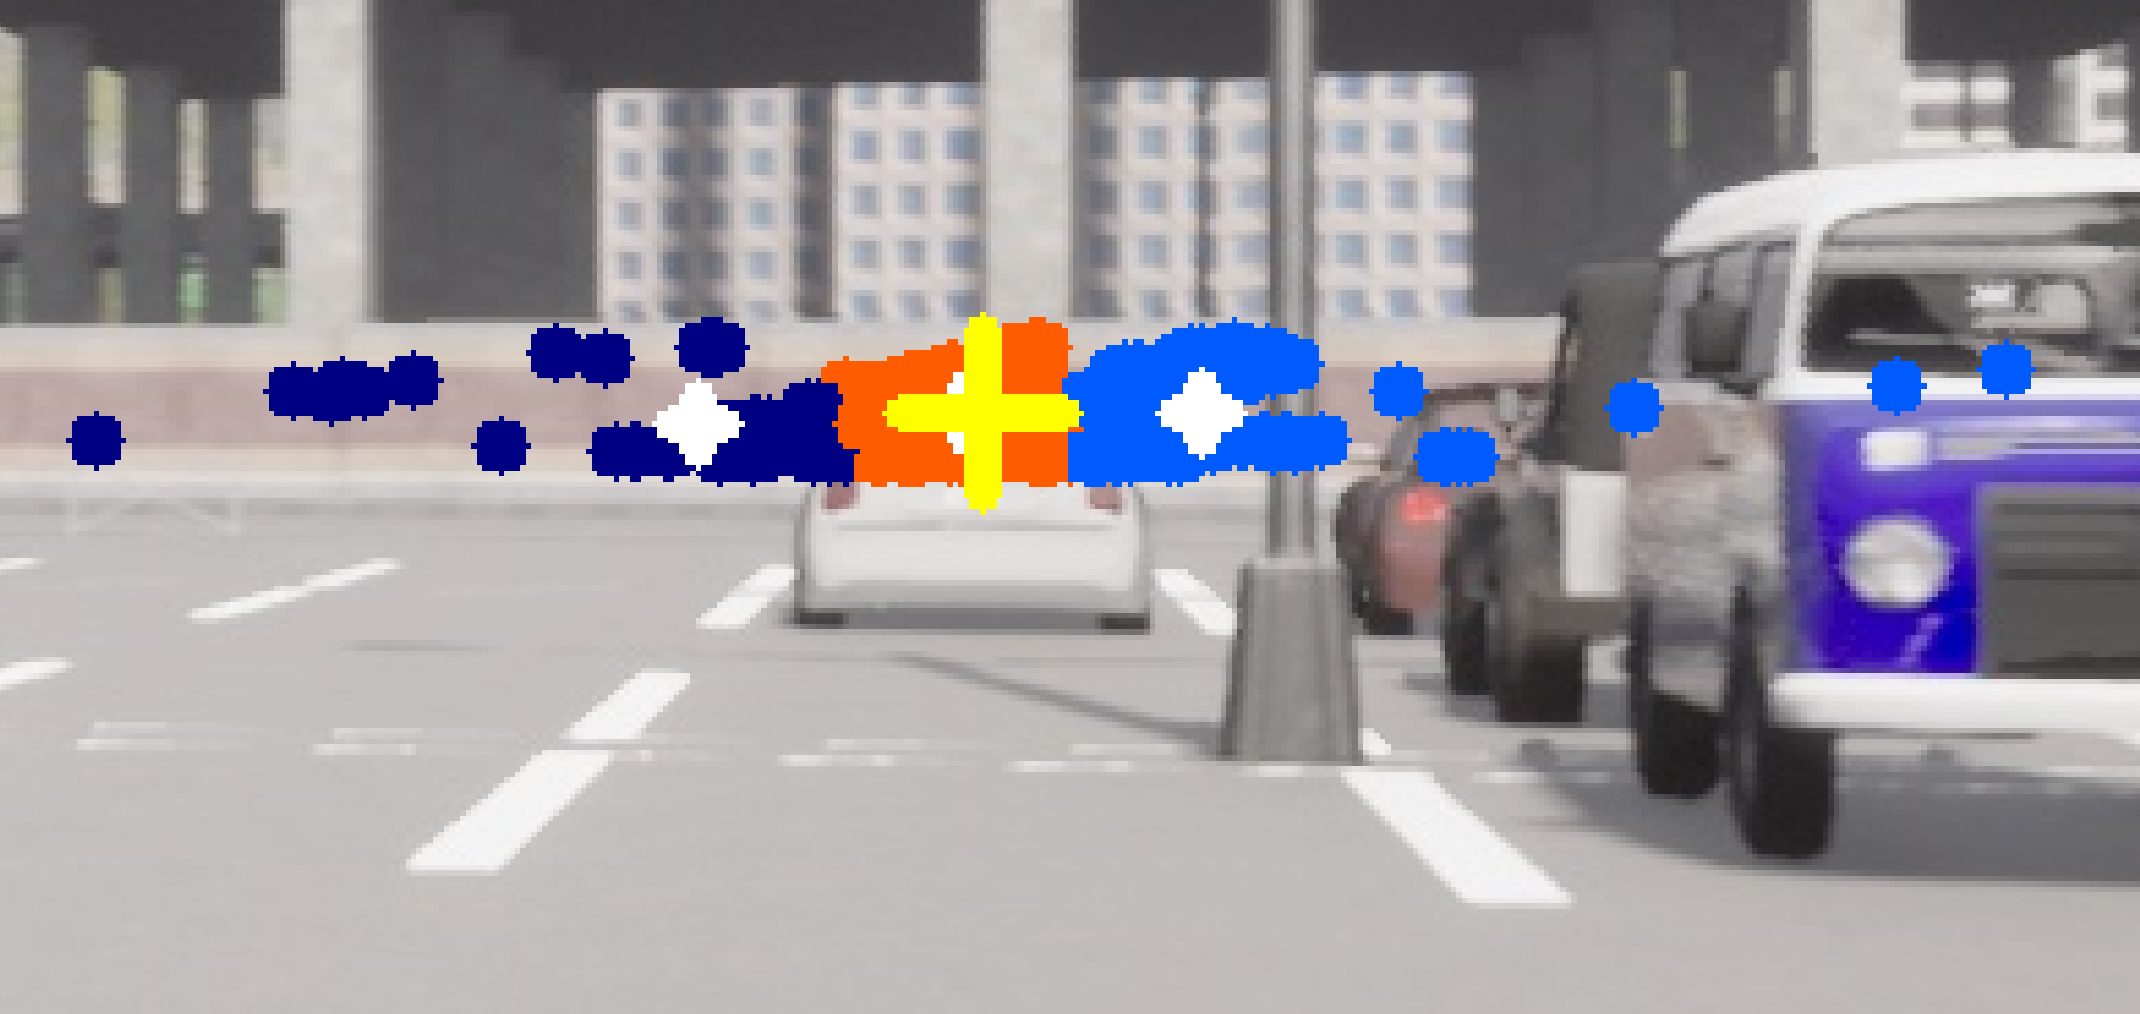
\includegraphics[width=0.9\textwidth]{img/reticule/vanishingPoint}
    \caption{Punto de fuga principal estimado}
    \label{fig:vanishingPoint}
\end{figure}

\subsubsection{Selección del 2do punto de fuga principal:}
\noindent
Una vez estimado el primer punto de fuga \(\mathbf{v}_1=(x_1,y_1)\), el segundo (\(\mathbf{v}_2\)) puede obtenerse
aprovechando que corresponde a una dirección ortogonal en 3D. Con un modelo pinhole simple, pixeles cuadrados, punto principal
en el centro \(C_x\), los puntos de fuga de direcciones ortogonales verifican la relación
\( (x_1-C_x)(x_2-C_x) + f^2 \approx 0 \). De ahí se despeja la coordenada horizontal de \(\mathbf{v}_2\):
\begin{equation}
    x_2 = C_x - \frac{f^2}{\,x_1 - C_x\,}, \qquad y_2 = y_1.
\end{equation}
Aquí \(f\) es la longitud focal en píxeles, que aproximamos a partir del FOV horizontal y el ancho de imagen \(W\):
\( f = \dfrac{W}{2\,\tan(\tfrac{\text{FOV}}{2})} \). En nuestro caso, con \(\text{FOV}=90^\circ\) y \(W=1920\), se fija
\(C_x=W/2\) y se calcula \(x_2\) como en la ecuación anterior, manteniendo \(y_2=y_1\) por pertenecer ambos a la misma línea del horizonte.

\subsubsection{Filtrado de intersecciones y líneas relevantes:}
\noindent
Una vez que se han identificado los puntos de fuga principales, se puede proceder a filtrar las intersecciones y las líneas que son
relevantes para la retícula de estacionamiento.
Primero, se filtran las intersecciones que están cerca de los puntos de fuga principales, utilizando un umbral de distancia que se puede ajustar experimentalmente.
Luego, se filtran las líneas que pasan por estas intersecciones relevantes.
Este proceso ayuda a eliminar el ruido y las líneas que no contribuyen a la formación de la retícula de estacionamiento.


\subsubsection{Mediciones en la retícula detectada:}
Pendiente de redacción.


\section{Ajuste de la retícula mediante RANSAC}\label{sec:metodo-ransac}
\noindent
Con base en los principios expuestos en la Sección \ref{sec:ransac-teorico},
aplicamos una adaptación de RANSAC para estimar una homografía que haga coherente una retícula ideal con
las líneas de los cajones visibles en la imagen. Este enfoque conserva la robustez frente a outliers y
oclusiones propias del escenario de estacionamiento.

\subsubsection{Variación de RANSAC para ajuste de retícula:}
\noindent
La variación propuesta sigue el ciclo de la Figura~\ref{fig:ramsac-flujo}:

\begin{figure}[!ht]
    \centering
    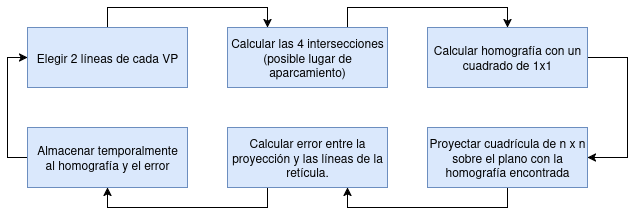
\includegraphics[width=0.99\textwidth]{img/3-metodo/ramsac-loop1.png}
    \caption{Esquema del ciclo RANSAC propuesto para el ajuste de la retícula.}
    \label{fig:ramsac-flujo}
\end{figure}

\noindent
Cada iteración del ciclo comprende los siguientes pasos:
\begin{enumerate}
    \item A partir de dos puntos de fuga estimados, agrupar las líneas detectadas en dos conjuntos según su punto de fuga asociado.
    \item Muestrear aleatoriamente dos líneas de cada conjunto y calcular las cuatro intersecciones \(P_1, P_2, P_3, P_4\) (producto cruzado de pares de rectas), que definen un candidato a cajón.
    \item Estimar la homografía \(\mathbf{H}\) que mapea el cuadrado canónico de lado 1 al cuadrilátero \(\{P_k\}_{k=1}^4\).
    \item Proyectar una retícula \(n\times n\) mediante \(\mathbf{H}\) sobre la imagen.
    \item Evaluar la consistencia entre la retícula proyectada y las líneas reales (por ejemplo, concordancia de orientación y proximidad en las regiones de soporte) y registrar una medida de ajuste.
    \item Almacenar temporalmente \(\mathbf{H}\) y su medida de ajuste; repetir desde el paso 2 durante \(N\) iteraciones.
\end{enumerate}

\noindent
Tras completar las iteraciones, se selecciona la homografía con mejor medida de consistencia 
como representación de la retícula en la imagen. 
Esta homografía permite extender el patrón más allá del campo visible, 
infiriendo la ubicación de cajones en puntos ciegos o parcialmente ocultos, 
lo que favorece la planificación de maniobras y el estacionamiento automático. 
Además, el esquema es robusto a líneas espurias y a oclusiones, 
y tiende a ser estable entre cuadros consecutivos al reutilizar la mejor homografía previa como
punto de partida (warm-start) . En la Figura~\ref{fig:ramsac-transform} se ilustra 
la transformación de un cuadrado canónico a un cajón detectado en la imagen mediante la homografía estimada.


\begin{figure}[!ht]
    \centering
    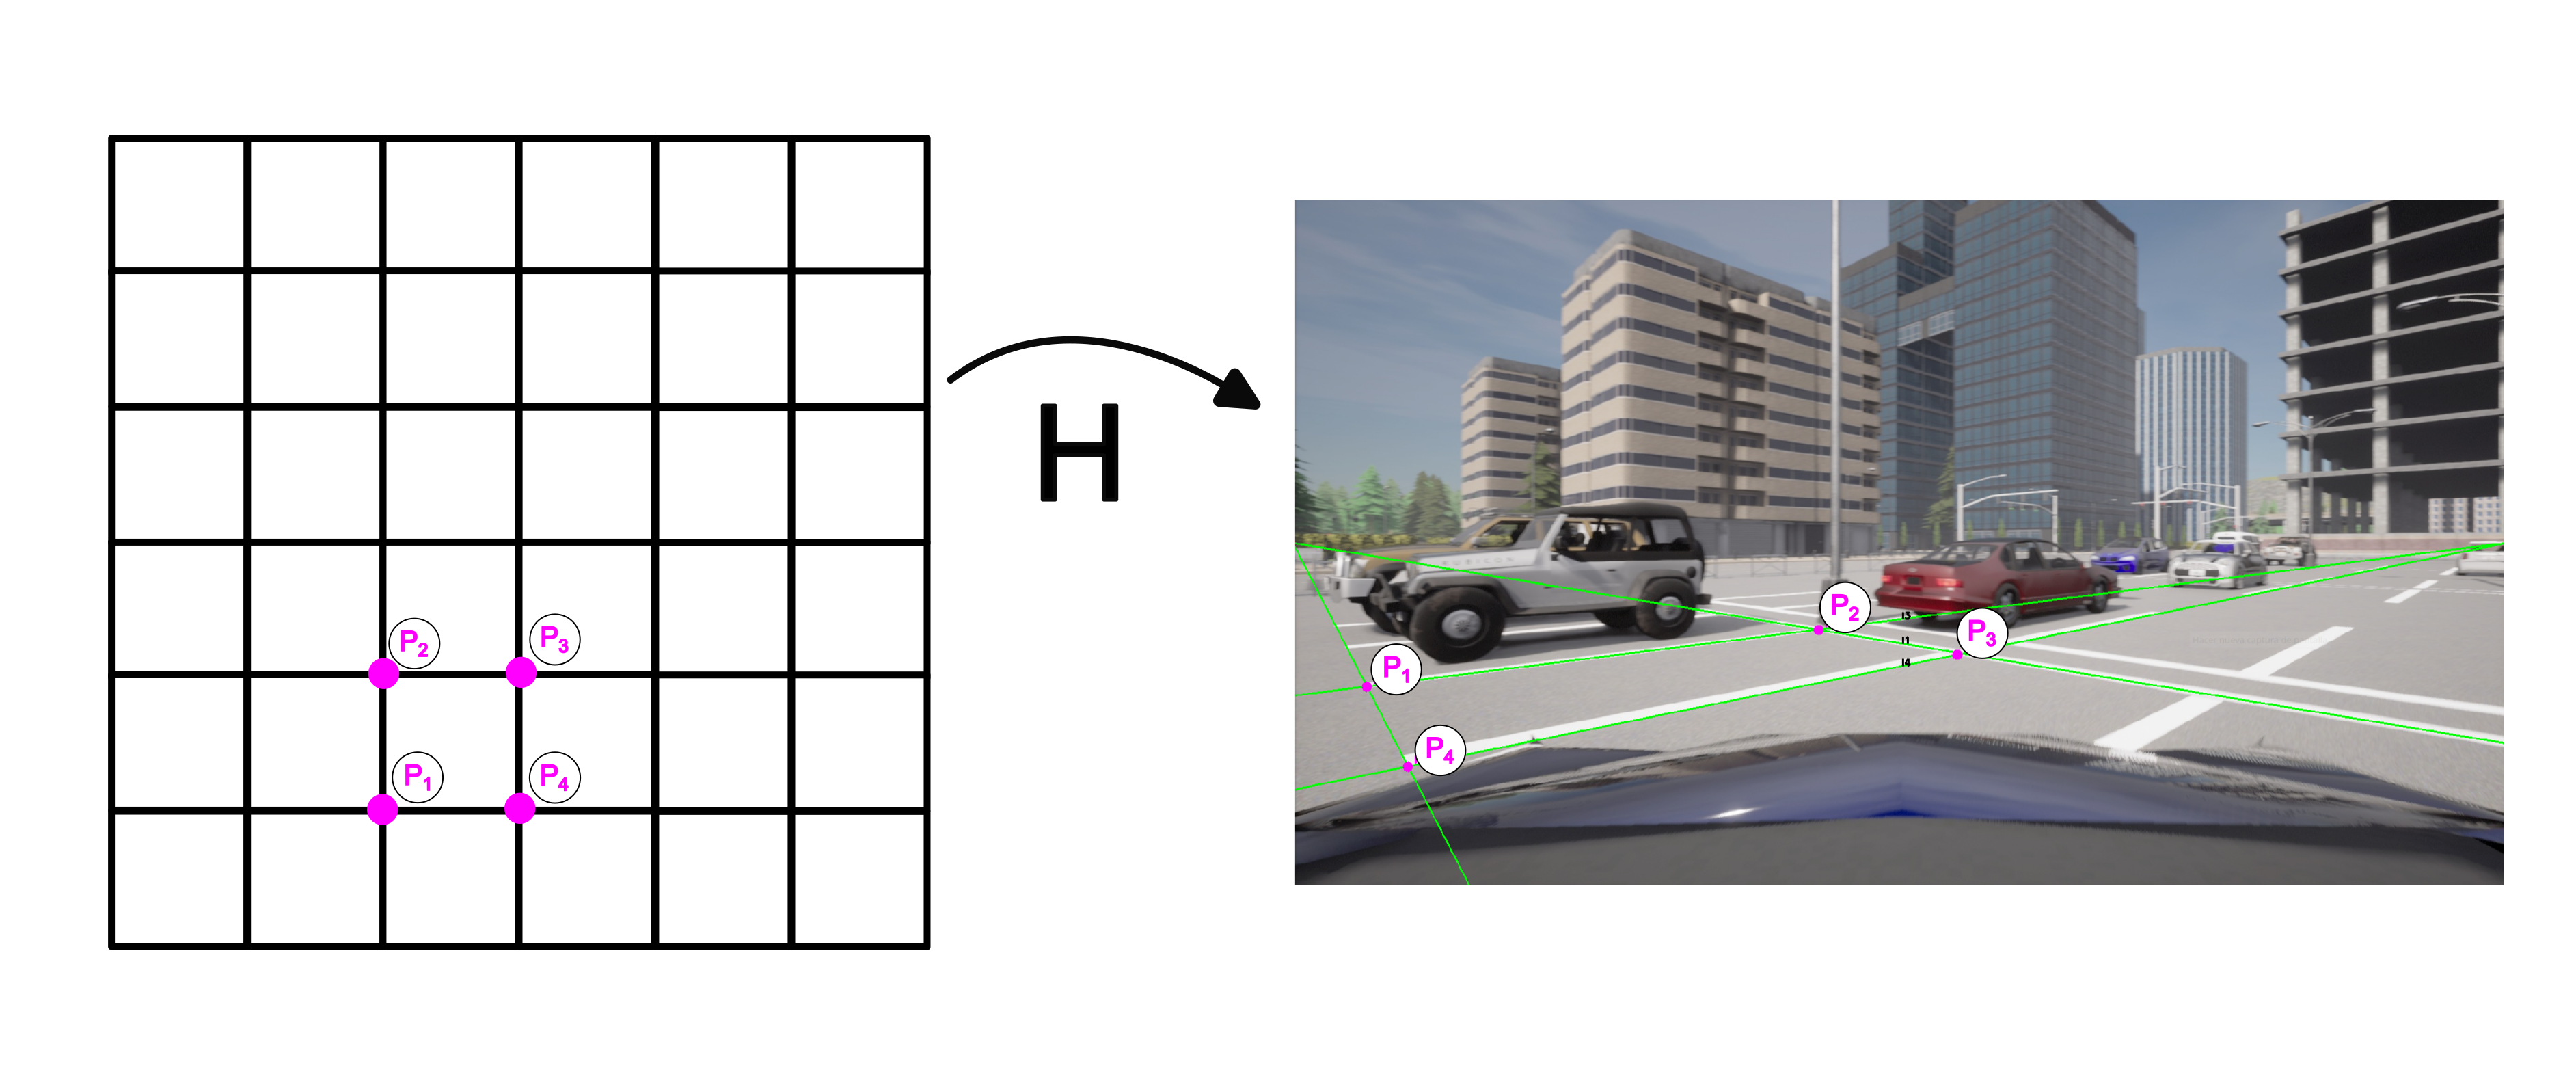
\includegraphics[width=0.99\textwidth]{img/3-metodo/transformacion.png}
    \caption{Estimación de una homografía \(\mathbf{H}\) que mapea un cuadrado canónico (izquierda) a un cuadrilátero de un cajón detectado en la imagen (derecha), permitiendo proyectar una retícula coherente aun cuando ciertas marcas no sean visibles.}
    \label{fig:ramsac-transform}
\end{figure}

\subsubsection{extracción de coordenadas en la retícula detectada:}
Pendiente de redacción.


% Capítulo 4: Resultados
\clearpage
\chapter{Resultados y aplicaciones}
Pendiente de redacción.
\section{Retículas obtenidas para diferentes escenarios}
Pendiente de redacción.

\section{Aplicación en aprendizaje por refuerzo}
\noindent
En esta sección demostramos la aplicación práctica de los conceptos de aprendizaje por refuerzo
(Sección~\ref{subsec:rl-components}) al problema de estacionamiento automático, utilizando
los resultados de detección de retícula obtenidos mediante las técnicas de visión por computadora
desarrolladas en este trabajo.

\subsubsection{Configuración del entorno con Gymnasium y CARLA}\label{subsec:rl-environment}
\noindent
Implementamos el entorno de aprendizaje por refuerzo utilizando \texttt{Gymnasium} como framework
estándar para la interfaz agente-entorno, integrado con el simulador CARLA que proporciona
un mundo físicamente realista. Esta combinación nos permite:

\begin{itemize}
    \item \textbf{Entorno físico}: CARLA simula las leyes de la física vehicular, incluyendo
    dinámica de carrocería, fricción de neumáticos, y colisiones realistas en el contexto
    de un estacionamiento con cajones delimitados.
    
    \item \textbf{Sensorización virtual}: El vehículo simulado está equipado con sensores
    que replican los de un vehículo real: cámara frontal, velocímetro, y sensores de pose.
    
    \item \textbf{Interfaz estandarizada}: Gymnasium proporciona la API estándar que permite
    intercambiar diferentes algoritmos de RL sin modificar el código del entorno.
\end{itemize}

\subsubsection{Definición del agente y espacio de acciones}\label{subsec:rl-agent}
\noindent
El agente implementa una política que mapea observaciones a acciones de control vehicular.
Siguiendo la terminología de la Sección~\ref{subsec:rl-components}, definimos:

\noindent
\textbf{Espacio de acciones}: Utilizamos un espacio continuo bidimensional
$\mathcal{A} = \text{Box}([-1, -1], [1, 1])$ donde cada acción $\mathbf{a} = [a_{\text{acc}}, a_{\text{dir}}]$ representa:
\begin{itemize}
    \item $a_{\text{acc}} \in [-1, 1]$: Control de aceleración. Valores positivos corresponden
    a aceleración hacia adelante, negativos a reversa, y cero a frenado.
    \item $a_{\text{dir}} \in [-1, 1]$: Control de dirección. Valores negativos giran a la izquierda,
    positivos a la derecha, y cero mantiene la dirección recta.
\end{itemize}

\subsubsection{Espacio de observaciones y sistema intérprete}\label{subsec:rl-observations}
\noindent
El estado del sistema se representa mediante un vector de observación $\mathbf{s} \in \mathbb{R}^6$:
\begin{equation}
    \mathbf{s} = [x, y, v_x, v_y, \cos(\theta), \sin(\theta)]
\end{equation}

donde:
\begin{itemize}
    \item $(x, y)$: Posición del vehículo en coordenadas del estacionamiento
    \item $(v_x, v_y)$: Componentes de velocidad
    \item $(\cos(\theta), \sin(\theta))$: Orientación del vehículo (representación continua del ángulo)
\end{itemize}

\noindent
\textbf{Sistema intérprete}: La estimación de posición y orientación $(x, y, \theta)$ se obtiene
aplicando los procedimientos de visión por computadora desarrollados en este trabajo:
detección de la retícula de estacionamiento (Sección~\ref{sec:metodo-reticula}) y
su ajuste mediante RANSAC (Sección~\ref{sec:metodo-ransac}). La velocidad se obtiene
directamente del sensor velocímetro del vehículo simulado.

\subsubsection{Adaptación del framework Highway-env}\label{subsec:rl-highway-adaptation}
\noindent
Para la implementación del aprendizaje por refuerzo adoptamos el framework Highway-env \cite{highway-env},
una biblioteca especializada en entornos de conducción autónoma que proporciona implementaciones
probadas y exitosas de espacios de acción, observación y funciones de recompensa para tareas
de estacionamiento. En lugar de desarrollar estos componentes desde cero, nos enfocamos en
integrar nuestra contribución de visión por computadora con esta solución establecida.

\noindent
\textbf{Contribución específica}: Nuestra aportación principal consiste en reemplazar el
sistema de observación simplificado de Highway-env por un intérprete realista basado en
los algoritmos de detección de retícula desarrollados en este trabajo, y migrar la
simulación del entorno abstracto original a CARLA para obtener una física vehicular
más precisa.

\noindent
\textbf{Componentes reutilizados de Highway-env}:
\begin{itemize}
    \item \textbf{Espacio de acciones}: $\mathcal{A} = \text{Box}([-1, -1], [1, 1])$ para control continuo [aceleración, dirección]
    \item \textbf{Función de recompensa}: Basada en distancia al objetivo con penalización de acciones bruscas
    \item \textbf{Estrategia de episodios}: Criterios de terminación y reinicio del entorno
\end{itemize}

\noindent
Los detalles completos del diseño original de Highway-env se describen en la
Sección~\ref{subsec:highway-env-theory}. En la siguiente sección analizaremos
la implementación específica y los resultados obtenidos con esta adaptación.

\subsubsection{Integración de visión por computadora y RL}\label{subsec:rl-integration}
\noindent
La contribución principal de este trabajo radica en la integración del sistema de
detección de retícula desarrollado como intérprete de observaciones en el framework
de aprendizaje por refuerzo. Mientras que Highway-env utiliza información de pose
perfecta y simplificada, nuestro sistema debe:

\begin{itemize}
    \item \textbf{Procesar imágenes reales}: Aplicar los algoritmos de Canny, Hough y RANSAC
    a la imagen de la cámara frontal del vehículo simulado en CARLA
    \item \textbf{Estimar pose}: Convertir la detección de retícula en estimaciones de
    posición $(x,y)$ y orientación $\theta$ del vehículo respecto al estacionamiento
    \item \textbf{Manejar incertidumbre}: Lidiar con detecciones imperfectas, oclusiones
    y condiciones de iluminación variables que no existen en el entorno abstracto original
\end{itemize}

\noindent
Esta integración permite evaluar la robustez y utilidad práctica de los algoritmos
de visión por computadora en una aplicación de control en tiempo real, demostrando
que es posible reemplazar sensores idealizados por sistemas de percepción basados
en cámara para tareas de navegación autónoma compleja.


\section{Highway-env aplicando la retícula detectada}
\noindent
En esta sección implementamos el modelo de aprendizaje por refuerzo combinando Highway-env con CARLA,
utilizando los resultados de detección de retícula como sistema de observación. La implementación
mantiene la estructura probada de Highway-env pero integra elementos realistas a través de wrappers
personalizados que conectan con el simulador CARLA y nuestro sistema de visión por computadora.

\subsubsection{Configuración del modelo}
\noindent
Utilizamos el algoritmo SAC (Soft Actor-Critic) de Stable-Baselines3 (Sección~\ref{sec:stable-baselines3})
con Hindsight Experience Replay (HER) para manejar la naturaleza de objetivo disperso del estacionamiento.
La configuración sigue las mejores prácticas de Highway-env (Sección~\ref{subsec:highway-env-theory}):

\begin{itemize}
    \item \textbf{Algoritmo}: SAC con política \texttt{MultiInputPolicy} para manejar espacios de observación estructurados
    \item \textbf{HER}: 4 objetivos muestreados por episodio con estrategia "future" para aprendizaje de objetivos dispersos
    \item \textbf{Hiperparámetros}: Buffer de 1M transiciones, learning rate 1e-3, red neuronal [256, 256, 256]
    \item \textbf{Entorno base}: \texttt{parking-v0} de Highway-env con modificaciones mediante wrappers
\end{itemize}

\subsubsection{Arquitectura de wrappers}
\noindent
Implementamos tres wrappers de Gymnasium (Sección~\ref{sec:gymnasium}) que adaptan el entorno original
manteniendo compatibilidad con la interfaz estándar:

\noindent
\textbf{CarlaInitRoadWrapper}: Construye la geometría del estacionamiento usando coordenadas reales de CARLA
(Sección~\ref{sec:carla-teorico}). Reemplaza el \texttt{RoadNetwork} predeterminado con cajones de estacionamiento
generados a partir de la posición objetivo actual en el simulador, creando un layout de 7 cajones centrado
en el objetivo.

\noindent
\textbf{CarlaObservationWrapper}: Sustituye las observaciones idealizadas de Highway-env por estimaciones
realistas obtenidas mediante nuestro sistema de visión por computadora. Aplica los algoritmos de detección
de retícula desarrollados (Sección~\ref{sec:metodo-reticula}) para extraer coordenadas $(x,y)$ y orientación
$\theta$ del vehículo, complementadas con velocidad del sensor vehicular de CARLA.

\noindent
\textbf{CarlaActionWrapper}: Traduce las acciones continuas $[aceleración, dirección]$ del agente de RL
a controles vehiculares en CARLA, aplicando throttle y steering al vehículo simulado y sincronizando
el tiempo de simulación.

\subsubsection{Integración del sistema de visión}
\noindent
El componente crítico de nuestra adaptación reside en el \texttt{CarlaObservationWrapper}, que implementa
el pipeline completo de visión por computadora como intérprete de observaciones:

\begin{enumerate}
    \item \textbf{Captura de imagen}: Obtiene el frame de la cámara frontal del vehículo en CARLA
    \item \textbf{Detección de retícula}: Aplica los algoritmos desarrollados (Canny, Hough, RANSAC)
    para identificar la estructura del estacionamiento
    \item \textbf{Estimación de pose}: Convierte la retícula detectada en coordenadas del vehículo
    relativas al estacionamiento mediante el procedimiento descrito en la metodología
    \item \textbf{Construcción de observación}: Formatea las estimaciones en el vector de estado
    esperado por el agente de RL: $[x, y, v_x, v_y, \cos(\theta), \sin(\theta)]$
\end{enumerate}

\noindent
Esta integración permite que el agente aprenda políticas de estacionamiento basándose en información
visual procesada en tiempo real, replicando las condiciones que enfrentaría un sistema autónomo real
donde la localización debe inferirse de sensores imperfectos en lugar de coordenadas globales ideales.

\subsubsection{Ventajas de la implementación híbrida}
\noindent
La arquitectura propuesta combina las fortalezas de cada componente:
\begin{itemize}
    \item \textbf{Highway-env}: Funciones de recompensa validadas y convergencia probada de algoritmos
    \item \textbf{CARLA}: Física vehicular realista y renderizado visual de alta fidelidad
    \item \textbf{Sistema de visión}: Percepción basada en cámara con incertidumbre realista
    \item \textbf{Gymnasium/SB3}: Interfaz estándar y algoritmos de RL de última generación
\end{itemize}

\noindent
Esta configuración permite evaluar tanto la robustez del sistema de detección de retícula
como su viabilidad en aplicaciones de control autónomo, demostrando que es posible sustituir
sensores idealizados por sistemas de percepción visual en tareas complejas de navegación.


\subsection{Comparación de resultados}

% Capítulo 4: Conclusiones y trabajo futuro
\clearpage
\chapter{Conclusiones y trabajo futuro}
Pendiente de redacción .

\end{linespacing}
% Referencias
\clearpage
\bibliographystyle{acm}
\bibliography{references}

\end{document}